%\documentclass[handout]{beamer}
\documentclass{beamer}
\usepackage[ruled,linesnumbered]{algorithm2e}
\usepackage{natbib}
%\usepackage{enumitem}
\definecolor{vuborange}{rgb}{1.0,0.40,0.0}
\usetheme{Boadilla}
\usepackage{amsmath,amssymb}
\usepackage{booktabs}
\title{Efficiently Explaining CSPs with Unsatisfiable Subset Optimization}
\institute[shortinst]
{\inst{1} Vrije Universiteit Brussel, Belgium \\ % Your institution for the title page
	\inst{2} KULeuven, Belgium \\ % Your institution for the title page
	\href{mailto:emilio.gamba@vub.be}{\underline{emilio.gamba@vub.be}}, \href{mailto:bart.bogaerts@vub.be}{bart.bogaerts@vub.be}, \href{mailto:tias.guns@kuleuven.be}{tias.guns@kuleuven.be} % Your email address
}
\date{IJCAI 2021}

\author{\underline{Emilio Gamba}\inst{1} \and  Bart Bogaerts\inst{1} \and   Tias Guns\inst{1,2}}

\newcommand\m[1]{\ensuremath{\mathcal{#1}}\xspace}
\newcommand\allconstraints{\m{T_P}}
\newcommand\formula{\ensuremath{\m{F} }\xspace}
\newcommand\formulac{\ensuremath{\m{C} }\xspace}
\renewcommand\emph[1]{{\color{vuborange}#1}}
\newcommand\Iend{\m{I_{\mathit{end}}}}
\newcommand\Ipartial{\m{I}}
 
 \newcommand\nat{\m{\mathbb{N}}}
 \newcommand\subsetT{\m{\mathcal{S}}}
 \newcommand\ltrue{\m{\textbf{t}}}
 \newcommand\lfalse{\m{\textbf{f}}}
 	\newcommand\call[1]{\m{\textsc{#1}}}
 \newcommand\onestep{\call{OneStep}}
 
\makeatletter
\setbeamertemplate{footline}
{
	\leavevmode%
	\hbox{%
		\begin{beamercolorbox}[wd=.2\paperwidth,ht=2.25ex,dp=1ex,center]{author in head/foot}%
			\usebeamerfont{author in head/foot}Emilio Gamba (VUB)
		\end{beamercolorbox}%
		\begin{beamercolorbox}[wd=.6\paperwidth,ht=2.25ex,dp=1ex,center]{title in head/foot}%
			\usebeamerfont{title in head/foot}Efficiently Explaining CSPs with Unsatisfiable Subset Optimization
		\end{beamercolorbox}%
		\begin{beamercolorbox}[wd=.2\paperwidth,ht=2.25ex,dp=1ex,right]{date in head/foot}%
			\usebeamerfont{date in head/foot}August 2021\hspace*{1em}
%			\insertframenumber{} / \inserttotalframenumber\hspace*{2ex} 
	\end{beamercolorbox}}%
	\vskip0pt%
}
\makeatother

\begin{document}
	
	\begin{frame}
	\maketitle
\end{frame}


	\AtBeginSection[]
	{
	\begin{frame}
		\frametitle{Outline}
		\tableofcontents[currentsection]
	\end{frame}
	}

	\AtBeginSubsection[]
	{
		\begin{frame}
			\frametitle{Outline}
			\tableofcontents[currentsection,currentsubsection]
		\end{frame}
	}
%	\begin{frame}
%		\frametitle{Outline}
%		
%		\begin{enumerate}
%			\item Background
%			\item Motivation
%			\item Contributions
%			\begin{enumerate}
%				\item {\color{vuborange}Optimality}
%				\item {\color{vuborange}Constrainedness}
%				\item {\color{vuborange}Incrementality}
%			\end{enumerate}
%			\item Applications
%			\item Results
%			\item Conclusion
%			\item Ideas for future work
%		\end{enumerate}
%	\end{frame}
	
	\begin{frame}
	\frametitle{Examples of Constraint Satisfaction Problems}
		\begin{minipage}[t]{0.6\textwidth}
			\begin{figure}[h]
				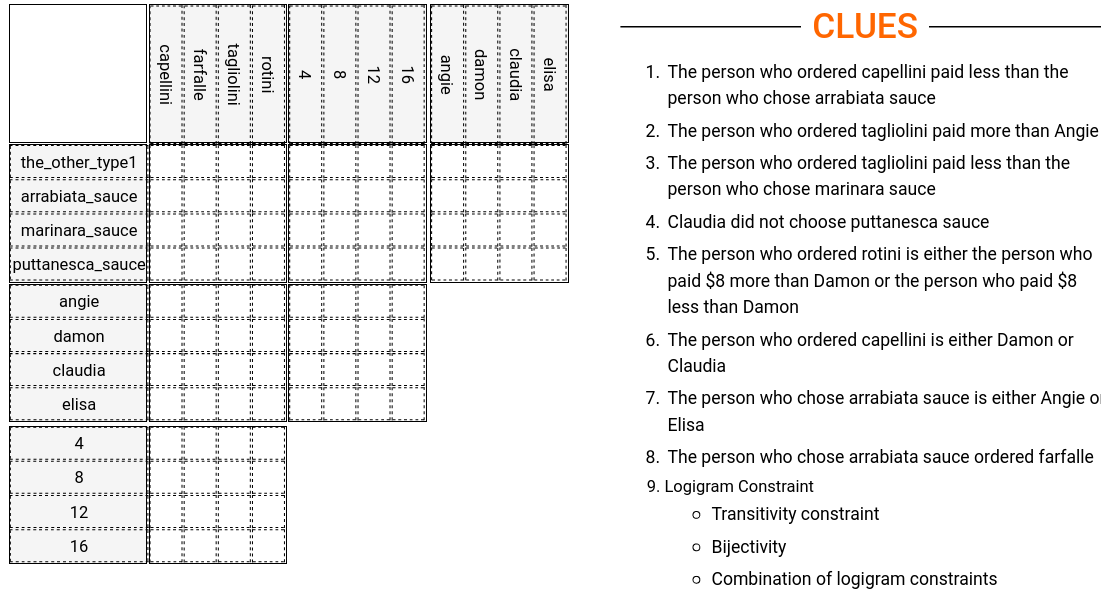
\includegraphics[width=\textwidth]{figures/logic_puzzle.png}
				\caption{Logic grid puzzle: Pasta Puzzle}
			\end{figure}
		\end{minipage}
	\hfill
			\begin{minipage}[t]{0.29\textwidth}
			\begin{figure}[h]
				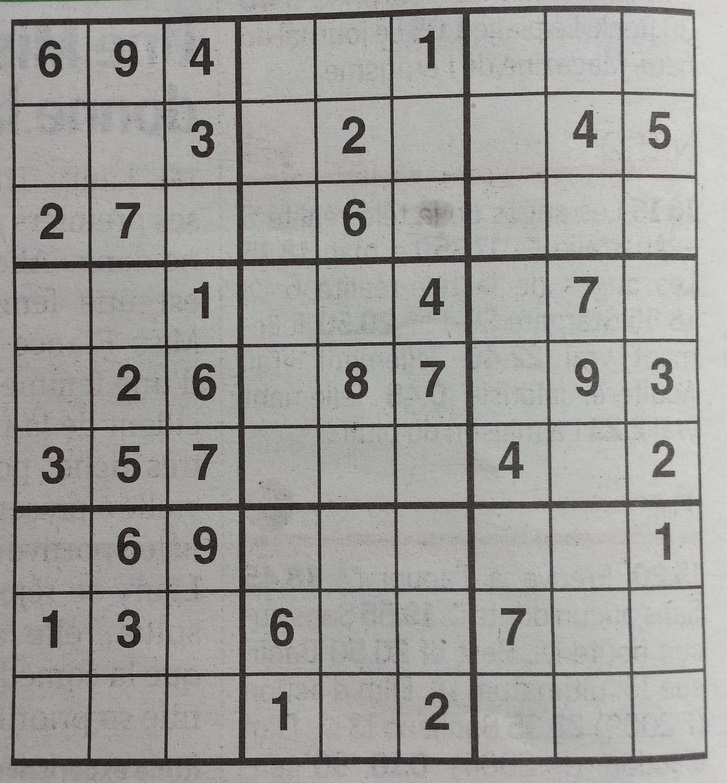
\includegraphics[width=\textwidth]{figures/sudoku.jpg}
				\caption{Sudoku}
			\end{figure}
		\end{minipage}
	\end{frame}


	\begin{frame}
		\frametitle{Outline}
		\tableofcontents
	\end{frame}

	\section{Background}
	\begin{frame}{Background}
	\framesubtitle{Context}
	In \cite{bogaerts2020step}, we proposed:\pause

		\begin{itemize}
			\item Step-wise explanation problem
			\item Algorithm 
			\item Heuristics for guiding the search for explanations
		\end{itemize}
		\end{frame}

%	\begin{frame}{Background}
%	\framesubtitle{Notation for CSPs}
%%	In \cite{bogaerts2020step}, we proposed a method for step-wise explaining solutions of Constraint Satisfaction Problems (CSPs):\pause
%	\begin{description}
%		\item[$\Sigma$] Propositional vocabulary% constraints over variables $V$ with domains $D$
%		\item[$\m{C}$] Propositional theory (set of constraints over $\Sigma$)% 
%		\begin{itemize}
%			\item \textit{\emph{notation}}: set of constraints (conjunction)
%		\end{itemize}
%		\item[$\m{I}$] (partial) interpretation (partial solution): consistent set of literals over $\Sigma$
%		\begin{itemize}
%			\item \textit{\emph{notation}}: set of (unit) clauses
%		\end{itemize}
%		\item[$\m{C} \wedge \m{I} \models \m{I}'$] Consequence of a theory given an interpretation
%	%		\item[$f$] a cost-function quantifying the difficulty of an explanation step\pause
%%		\item[$\m{I}_{end}$] interpretation-to-explain (solution) of the CSP \pause  
%%		\item[$\m{I}_{end} \setminus \m{I}$] remaining facts to explain
%	\end{description}
%
%%	\begin{definition}
%%		An \emph{\color{vuborange}explanation} is defined as a \textit{sequence} of simple inference steps.
%%	\end{definition}\pause
%	\end{frame}
%
%	\begin{frame}{Background}
%	\framesubtitle{Goal}
%	Given $\mathbf{\m{C}}$ and $\mathbf{\m{I}}$, let $\Iend$ the maximal set of literals s.t.
%	\[\m{C} \land \m{I} \models \Iend\]
%		\begin{itemize}
%		    \item Explain in simple steps how to derive \Iend
%			\item Our focus: single steps  (not optimizing entire sequence yet)
%		\end{itemize}
%	\end{frame}
%
%	\begin{frame}{Background}
%		\framesubtitle{\cite{bogaerts2020step}: Formalizing Explanations}
%		\begin{definition}
%			\small
%			Let $\m{I}_{i-1}$ and $\m{I}_i$ be partial interpretations such that $\m{I}_{i-1}\wedge \m{C} \models \m{I}_i$.
%			We say that $(E_i,S_i,N_i)$ \emph{explains} the derivation of $\m{I}_{i}$ from $\m{I}_{i-1}$ if the following hold:
%			\begin{itemize}
%				\item \emph{$N_i$} $= \m{I}_i \setminus \m{I}_{i-1}$ (i.e., $N_i$ consists of all newly defined facts), \pause
%				\item \emph{$E_i$} $\subseteq \m{I}_i$ (i.e., the explaining facts are a subset of what was previously derived),\pause
%				\item \emph{$S_i$} $ \subseteq \m{C}$ (i.e., a subset of the clues and implicit constraints are used), and \pause
%				\item \emph{$S_i \land E_i \models N_i$} (i.e., all newly derived information indeed follows from this explanation).
%			\end{itemize}
%		\end{definition}\pause
%			 \begin{definition}
%		\small
%		We call $(E_i,S_i,N_i)$ a \emph{non-redundant explanation of  the derivation of $\m{I}_i$ from $\m{I}_{i-1}$} if it explains this derivation and whenever $E'\subseteq E_i; S'\subseteq S_i$ while $(E',S',N_i)$ also explains this derivation, it must be that $E_i=E', S_i=S'$. 
%	\end{definition}
%	\end{frame}
%
%	\begin{frame}{Background}
%		\framesubtitle{\cite{bogaerts2020step}: Explaining how to solve Constraint Satisfaction Problems}
%%		\begin{definition}
%%			An \emph{\color{vuborange}explanation} is defined as a \textit{sequence} of simple inference steps. 
%%		\end{definition}\pause
%%		Given a formula $\m{C}$, a partial interpretation $\m{I}$, a new fact $\ell \in {\Iend} \setminus \m{I}}$ 
%%		 \begin{definition}
%%		 	\small
%%			We call $(E_i,S_i,N_i)$ a \emph{non-redundant explanation of  the derivation of $\m{I}_i$ from $\m{I}_{i-1}$} if it explains this derivation and whenever $E'\subseteq E_i; S'\subseteq S_i$ while $(E',S',N_i)$ also explains this derivation, it must be that $E_i=E', S_i=S'$. 
%%		\end{definition}
%%	
%
%		 \textit{Observation:} computing non-redundant explanations of a single literal can be done using Minimal Unsat Core (MUS) extraction:\pause
%		\begin{theorem}
%			\small
%			There is a one-to-one correspondence between $\subseteq-$minimal unsatisfiable cores of $\m{C} \wedge \m{I}_i \wedge \lnot \ell$. and non-redundant explanations of $\m{I}_i \cup \{\ell\}$ (given $\m{C}$)
%		\end{theorem}\pause
%%	}
%Furthermore, we assume existence of a \emph{cost function} $f(E_i,S_i,N_i)$ that quantifies the interpretability of a single explanation
%	
%%	\begin{block}{Explanation sequence generation problem}
%%		Find a \emph{non-redundant} explanation sequence that explains all derivations need to solve the CSP.
%%	\end{block}\pause
%	\end{frame}
%
%%		\begin{frame}{Background}
%%			\framesubtitle{Explaining how to solve Constraint Satisfaction Problems}
%%		%		\begin{definition}
%%		%			An \emph{\color{vuborange}explanation} is defined as a \textit{sequence} of simple inference steps. 
%%		%		\end{definition}\pause
%%		%		Given a formula $\m{C}$, a partial interpretation $\m{I}$, a new fact $\ell \in {\Iend} \setminus \m{I}}$ 
%%		\begin{definition}
%%			\small
%%			We call $(E_i,S_i,N_i)$ a \emph{non-redundant explanation of  the derivation of $I_i$ from $I_{i-1}$} if it explains this derivation and whenever $E'\subseteq E_i; S'\subseteq S_i$ while $(E',S',N_i)$ also explains this derivation, it must be that $E_i=E', S_i=S'$. 
%%		\end{definition}\pause
%%	Furthermore, we assume existence of a \emph{cost function} $f(E_i,S_i,N_i)$ that quantifies the interpretability of a single explanation
%%
%%	\end{frame}
%
%
%	\begin{frame}{Background}
%		\framesubtitle{\cite{bogaerts2020step}: Formalizing non-redundant explanation sequences}
%		\begin{definition}
%				\small
%			Given a theory $\m{C}$ and initial partial interpretation $\m{I}_0$, the \emph{explanation-production problem} consist of finding a non-redundant explanation sequence
%			\[ \langle \hspace{3pt}(\m{I}_0,(\emptyset,\emptyset,\emptyset))\hspace{3pt}, \hspace{3pt} (\m{I}_1,(E_1,S_1,N_i)) \hspace{3pt},\hspace{3pt} \dots \hspace{3pt}, \hspace{3pt}(\m{I}_n,(E_n,S_n,N_n)) \hspace{3pt}\rangle\]
%			such that some aggregate over the sequence $\left(f(E_i,S_i,N_i)\right)_{i\leq n}$ is minimized.
%		\end{definition} 
%	\end{frame}


	\setlength{\algomargin}{15pt}
	\begin{frame}{Background}
		\framesubtitle{\cite{bogaerts2020step}: MUS-Based Explanation Generation}
		%  TODO ALGORITHM FROM IJCAI MUS... 
		
		
			\begin{algorithm}[H]
				\caption{$\onestep(\m{C},f,\m{I},\Iend)$}
				\label{alg:oneStep}
				$X_{best} \gets \mathit{nil}$\;
				\For{$\ell \in \{\Iend \setminus I\}$}{
					$X \gets \emph{\call{MUS}{(\m{C} \land \m{I} \land \neg \ell)}}$\;
					\If{$f(X)<f(X_{best})$}{
						$X_{best} \gets X$\;
					}
				}
				\Return{$X_{best}$} 
			\end{algorithm}\pause
			\begin{alertblock}{Note}
					\small
			The cost-function is not encoded in the explanation computation, but in the explanation finding heuristic. There is \emph{no guarantee} that the non-redundant explanation is \emph{provably cost-optimal}!
		\end{alertblock}
	\end{frame}

%	\begin{definition}
%		\emph{\color{vuborange}Simplicity} of an explanation is measured by the number and types of constraints and facts used. 
%	\end{definition}

%		\begin{definition}
%	Given one or a subset of the constraints ( $S_i \subseteq T_P$  ) and facts we know ($E_i\subseteq \mathcal{I}_i$), an \textbf{explanation} is an implication of the form $E_i \wedge S_i  \implies N_i $, where $N_i$ is the new information from $S_i \cup E_i \models N_i$. \cite{bogaerts2020step}
%\end{definition}
%	


%	\begin{frame}{Motivation}
%		\framesubtitle{Step-wise Explanations of CSPs}
%		\cite{bogaerts2020step} proposed a method for step-wise explaining solutions of constraint satisfaction problems.\pause
%	
%		
%%		\begin{definition}
%%			\emph{\color{vuborange}Simplicity} of an explanation is measured by the number and types of constraints and facts used. 
%%		\end{definition}
%	\end{frame}

%	\begin{frame}{Motivation}
%	\framesubtitle{Optimal explanations}
%	
%	Let \emph{f} be a cost function quantifying explanation difficulty.
%	\begin{definition}
%		An \emph{\color{vuborange} optimal} explanation is \emph{f}. 
%	\end{definition}\pause
%	
%\end{frame}

\section{Motivation}
	\begin{frame}{Motivation}
		\framesubtitle{Challenges and open questions from \cite{bogaerts2020step}}

		\begin{description}[font=\color{vuborange}\itshape]
			\small
			\item[Optimality] Explanations not provably optimal, \emph{heuristically} found.
			\begin{itemize}
				\item MUS guarantees non-redundancy but ... not quality.
				\item MUS-based heuristic
				\item SMUS: $\#$-minimal (\cite{ignatiev2015smallest})
			\end{itemize} \pause
			\item[Efficiency] Explanation generation takes a lot of time. \pause
			\item[Constrainedness] Can we avoid looping over the literals when searching for the next best explanation ?\pause
			\item[Incrementality] Can we reuse information from an explanation call to another? 
		\end{description}
	\end{frame}
\section{The OCUS Problem (Hitting Set-based Algorithm)}



\subsection{Optimality}
	\begin{frame}{Optimality}
	\framesubtitle{Integrating the cost function in non-redundant explanation computation}
	\begin{definition}
			\small
		Let $\m{F}$ be a formula, $f:2^{\m{F}} \to \nat$ a cost function. We call %a set $U\subseteq \formulag$ a \emph{$p$-constrained $f$-OUS} of \formulag ($(p,f)$-OUS) \tias{what with the OCUS name here?} \bart{I propsoe to say. We call 
		$\mathcal{S} \subseteq \m{F}$ an \emph{OUS}$^*$ of $F$ (with respect to $f$) if \begin{itemize}                                      
			\item $\subsetT$ is unsatisfiable,
			%       \item $p(\subsetT)$ is true
			\item all other unsatisfiable $\mathcal{S}'\subseteq \m{F}$ satisfy $f(\mathcal{S}')\geq f(\mathcal{S})$.
		\end{itemize}
	\end{definition}
	$^*$ = \emph{Optimal} Unsatisfiable Subset


		\end{frame}
	
	\begin{frame}{OUS-Based Explanation Generation}

		\begin{center}
			\Large
			\textbf{Q}: How to compute OUSs?		
		\end{center}\pause
		%  TODO ALGORITHM FROM IJCAI MUS... 
		
		\begin{algorithm}[H]
			\caption{$\onestep(\m{C},f,\m{I},\Iend)$}
			\label{alg:oneStep}
			$X_{best} \gets \mathit{nil}$\;
			\For{\color{black}$\ell \in \{\Iend \setminus \m{I}\}$}{
				$X \gets \call{OUS}{(\m{C} \land \m{I} \land \neg \ell, \emph{f})}$\;
				\If{\color{black}$f(X)<f(X_{best})$}{
					$X_{best} \gets X$\;
				}
			}
			\Return{$X_{best}$} 
		\end{algorithm}
	\end{frame}

\subsection{Constrainedness}

\begin{frame}{Constrainedness}
	\framesubtitle{Beyond OUS-based explanations}
	\begin{itemize}
		\item The different iterations (for loop line 2)... very similar
		\item Can we exploit this? 
		\pause
		\item Essentially, the task at hand is: find a single unsatisfiable subset of 
		\[\m{C} \land \m{I} \land \bigvee_{\ell\in \Iend\setminus \m{I}}\lnot \ell\]
		that:
		\begin{itemize}
			\item Is optimal w.r.t.\ $f$
			\item Contains \emph{exactly one} literal $\lnot \ell$ with $\ell \in \Iend\setminus \m{I} $ (\emph{example!})
		\end{itemize}
		
	\end{itemize}	
\end{frame}
% 
\begin{frame}{Constrainedness}
	\framesubtitle{The OCUS problem}
	\begin{definition}
			\small
		Let $\formula$ be a formula, $f:2^{\formula} \to \nat$ a cost function and  $p$ a predicate $p: 2^{\formula}\to \{\ltrue,\lfalse\}$. We call %a set $U\subseteq \formulag$ a \emph{$p$-constrained $f$-OUS} of \formulag ($(p,f)$-OUS) \tias{what with the OCUS name here?} \bart{I propsoe to say. We call 
		$\subsetT \subseteq \formula$ an \emph{OCUS}$^*$ of \formula (with respect to $f$ and $p$) if \begin{itemize}                                      
			\item $\subsetT$ is unsatisfiable,
			\item $p(\subsetT)$ is true
			\item \emph{all other unsatisfiable $\subsetT'\subseteq \formula$ with $p(\subsetT')=\ltrue$ satisfy $f(\subsetT')\geq f(\subsetT)$}.
		\end{itemize}
	\end{definition}
	$^*$ = Optimal \emph{Constrained} Unsatisfiable Subset
\end{frame}


\newcommand\onestepo{\ensuremath{\call{explain-One-Step-ocus}}\xspace}
\begin{frame}{OCUS-Based explanation generation}
	\begin{algorithm}[H]
		\DontPrintSemicolon
		\caption{$\onestepo(\m{C},f,\m{I},\Iend)$}
		\label{alg:oneStepOCUS}
		$p \leftarrow$ exactly one of $\overline{\Iend\setminus \m{I}}$\;
		\Return{$\call{OCUS}(\m{C}\land \m{I}\land \overline{\Iend\setminus \m{I}}, f, p)$} 
	\end{algorithm}
\end{frame}


\newcommand\muses[1]{\textsc{mus}s(\m{#1})}
\newcommand\mcses[1]{\textsc{mcs}s(\m{#1})}
\begin{frame}{How to find OCUSs?}
	\begin{itemize}
		\item Hitting set--based algorithms: used for MaxSAT and SMUS 
		%   \item We extended this idea to OCUS
		
		\begin{theorem}\label{prop:MCS-MUS-hittingset}	\small
			%     Given an $ \formula$, let MUSes($\formula$), be the Minimal Unsatisfiable Subsets of F and MCSes($\formula$), be the Minimal Correction Subsets of F:
			%     
			A set  $\subsetT \subseteq \formula$ is a MCS of $ \formula$ iff  it is a \emph{minimal hitting set} of \muses{\formula}.\\
			%     \noindent
			A set  $\subsetT \subseteq \formula$ is a MUS of $ \formula$ iff  it is a \emph{minimal hitting set} of \mcses{\formula}.
		\end{theorem}
		\pause
		\item We extended this to OCUS: 
	\end{itemize}
	
\end{frame}

\newcommand\setstohit{\m{\mathcal{H}}}
\newcommand\grow{\call{Grow}}
\newcommand\sat{\call{SAT}}
\newcommand\comus{\call{ocus}}
\newcommand\cohs{\call{cost-optimal-hittingset}}

\begin{frame}{Hitting set--based OCUS}
	\begin{algorithm}[H]
		\DontPrintSemicolon
		$\setstohit  \gets \emptyset$ \; %\label{omus-line1} 
		\While{true}{
			$\subsetT \gets \cohs(\setstohit,f,p) $  \;%\tcp*{\small Find \textb    $\setstohit  \gets \setstohit  \cup \{  \formula \setminus \F''\}$ \;
			% f{optimal} solution}
			% \tcp{\small set with all unique clauses from hitting set}
			%     (sat?, $\kappa$) $\gets$ \texttt{SatSolver}($hs$)\;
			% \tcp{If SAT, $\kappa$ contains the satisfying truth assignment}
			% \tcp{IF UNSAT, $hs$ is the OUS }
			\If{ $\lnot \sat(\subsetT)$}{
				\Return{$\subsetT$} \;
			}
			$\subsetT \gets  \grow(\subsetT,\formula) $ \label{line:grow}\;
			$\setstohit  \gets \setstohit  \cup \{  \formula \setminus \subsetT\}$ \;
		}
		\caption{$\comus(\formula,f,p)$ }
		\label{alg:comus}
	\end{algorithm}
\end{frame}

\begin{frame}{Hitting set--based OCUS}
	\only<1>{
	\begin{figure}
		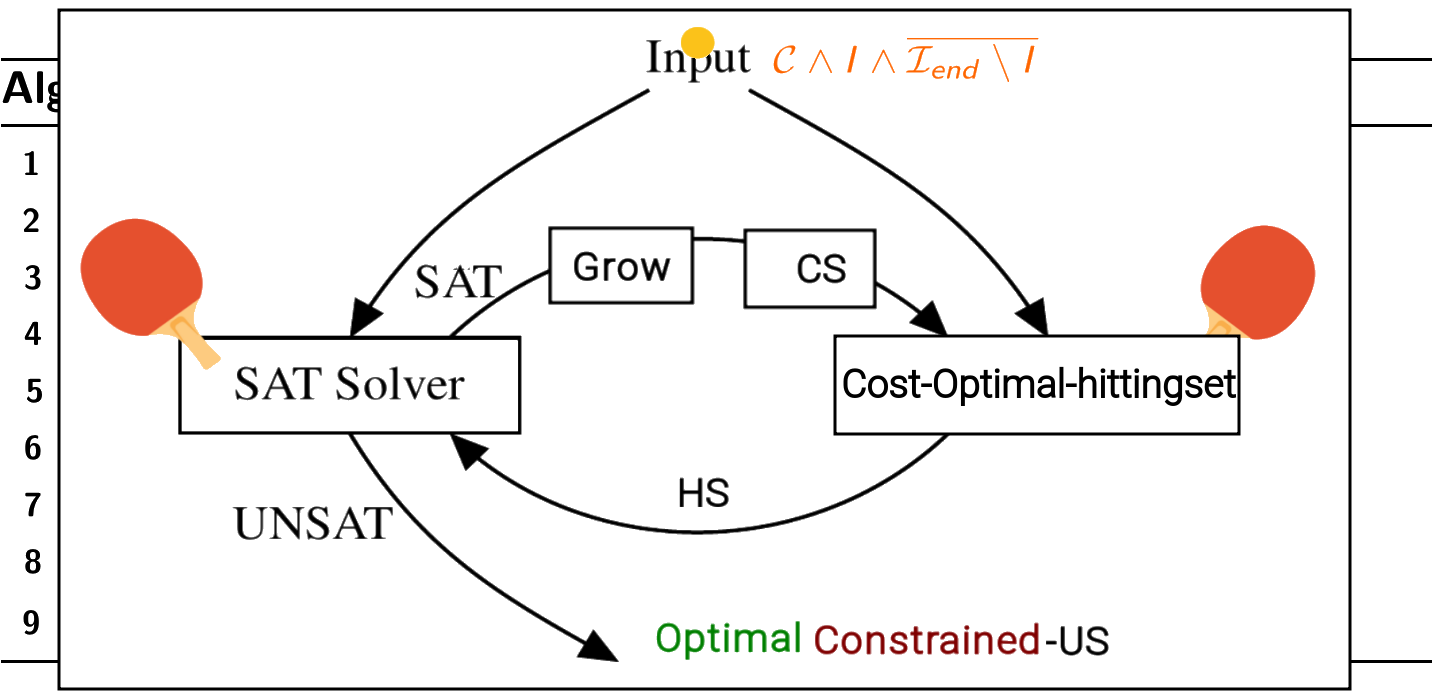
\includegraphics[width=\textwidth]{figures/algo_with_ping_pong0.png}
	\end{figure}
}
	\only<2>{
		\begin{figure}
			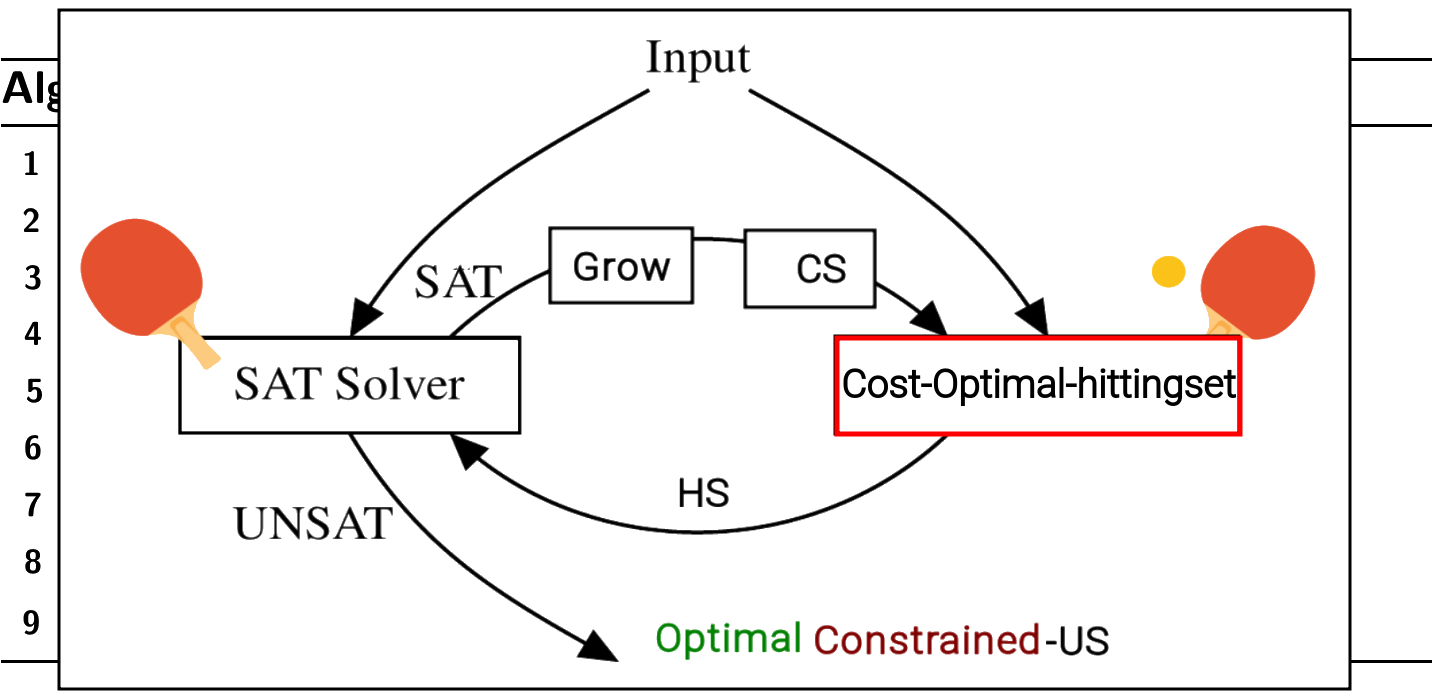
\includegraphics[width=\textwidth]{figures/algo_with_ping_pong.png}
		\end{figure}
	}
\only<3>{
		\begin{figure}
		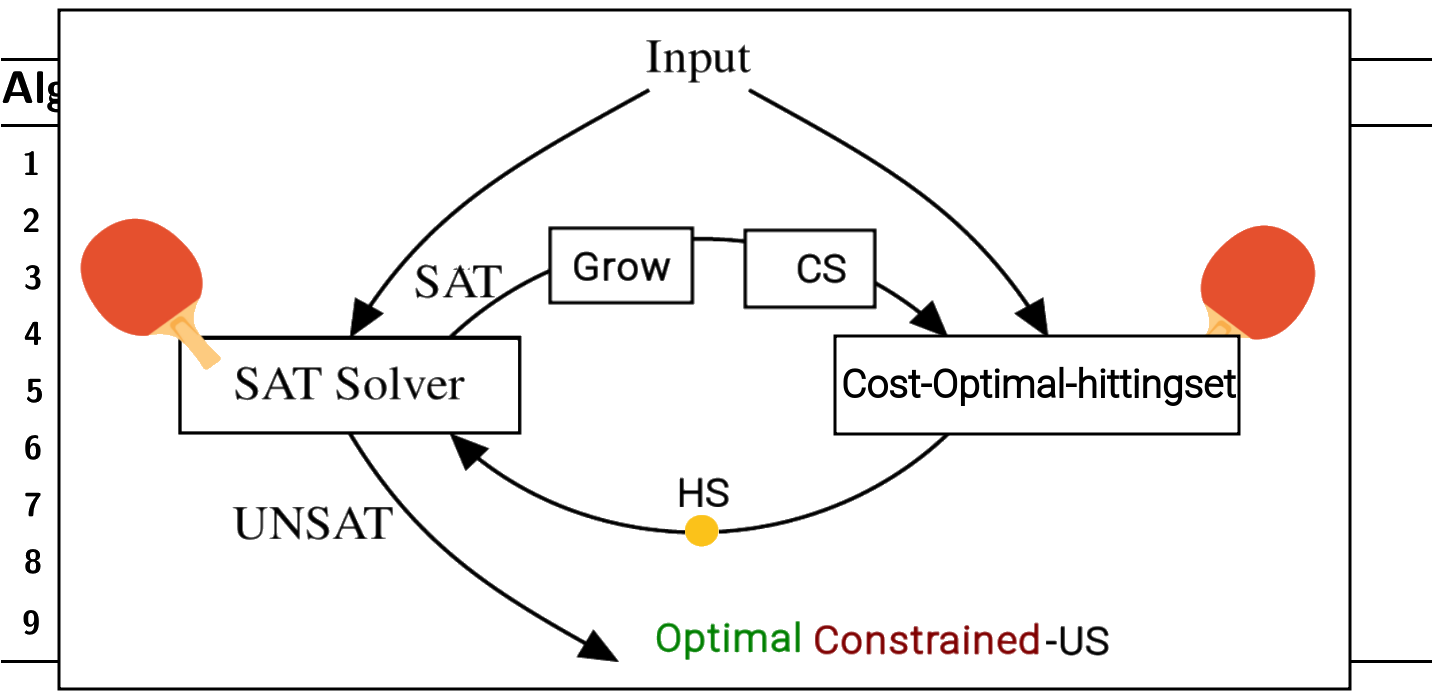
\includegraphics[width=\textwidth]{figures/algo_with_ping_pong1.png}
	\end{figure}
}
\only<4>{
		\begin{figure}
		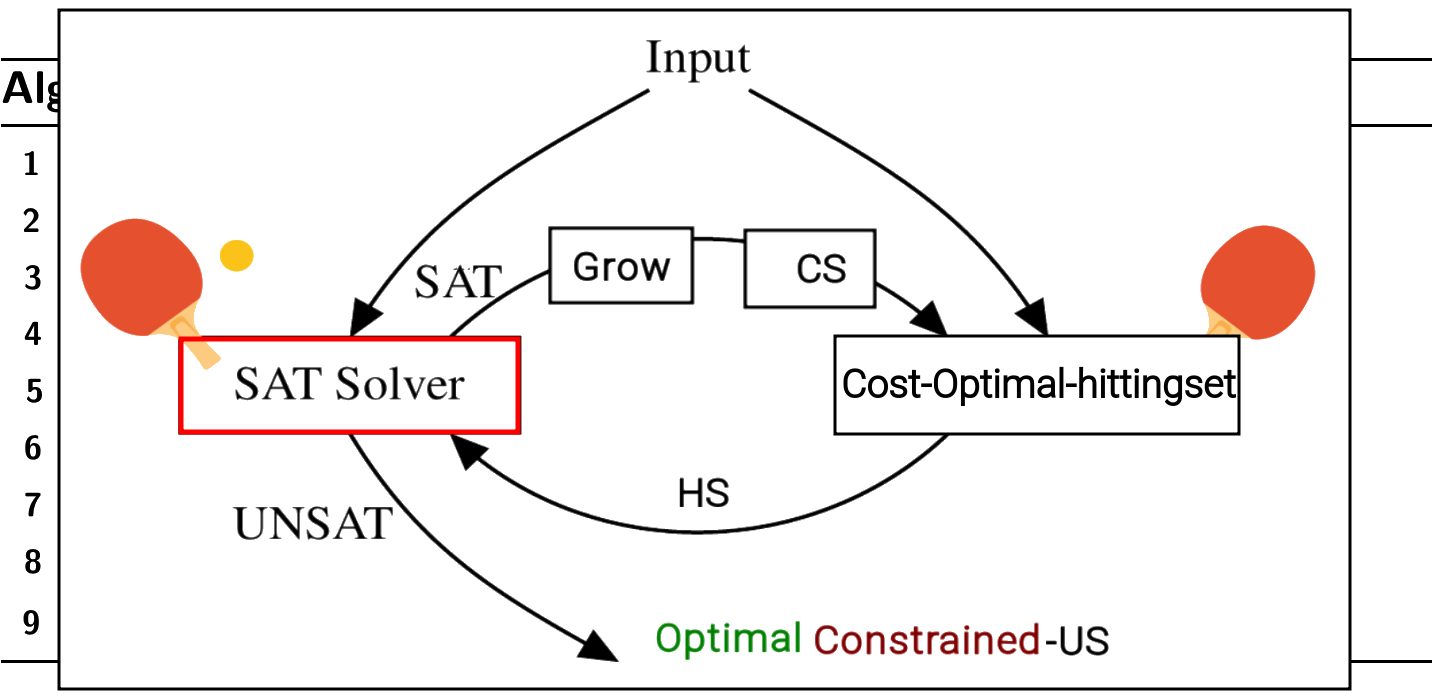
\includegraphics[width=\textwidth]{figures/algo_with_ping_pong2.png}
	\end{figure}
}
\only<5>{
		\begin{figure}
		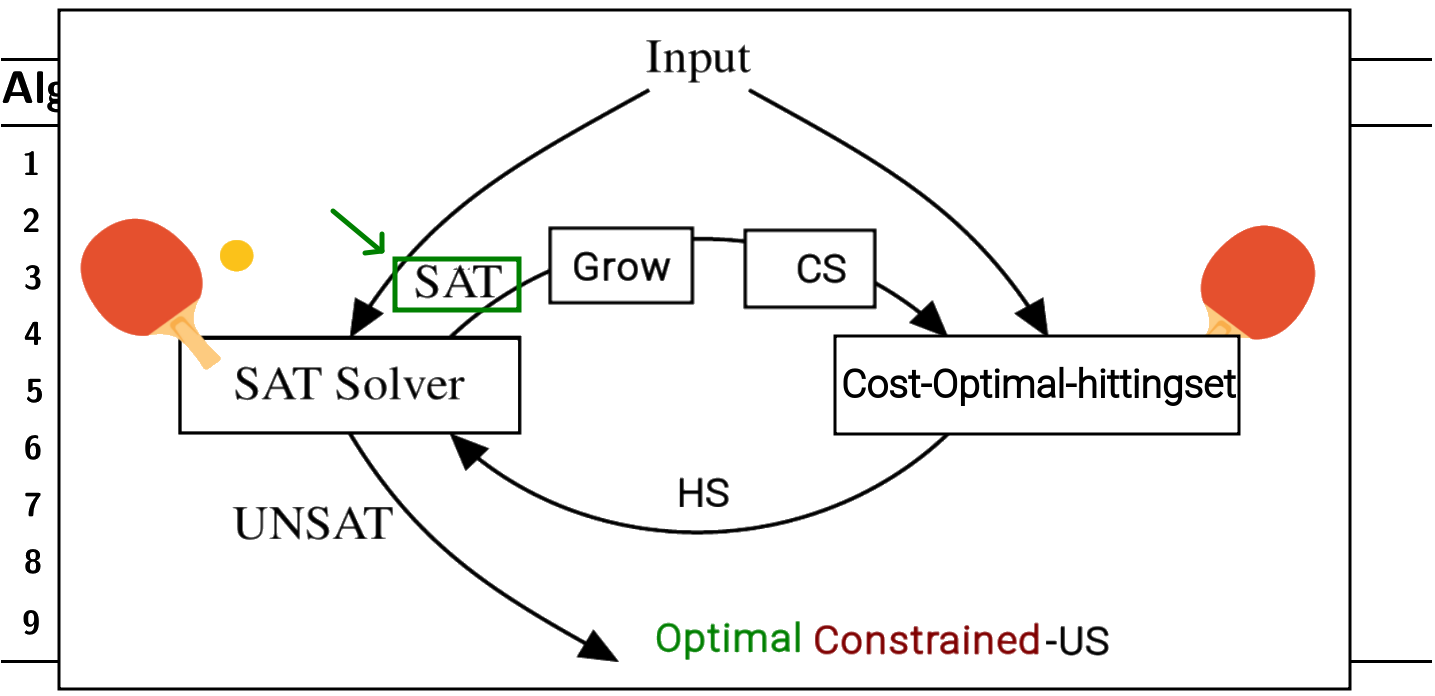
\includegraphics[width=\textwidth]{figures/algo_with_ping_pong2a.png}
	\end{figure}
}
\only<6>{
		\begin{figure}
		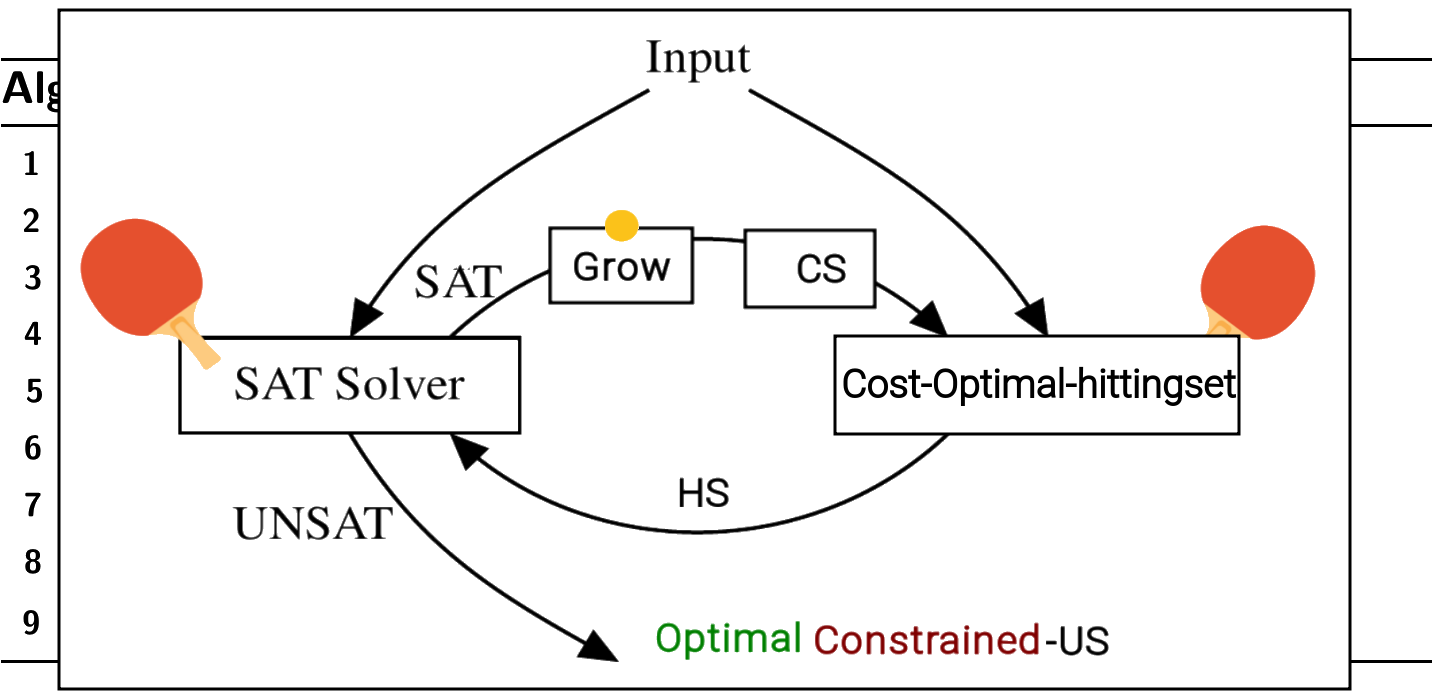
\includegraphics[width=\textwidth]{figures/algo_with_ping_pong2b.png}
	\end{figure}
}
\only<7>{
		\begin{figure}
		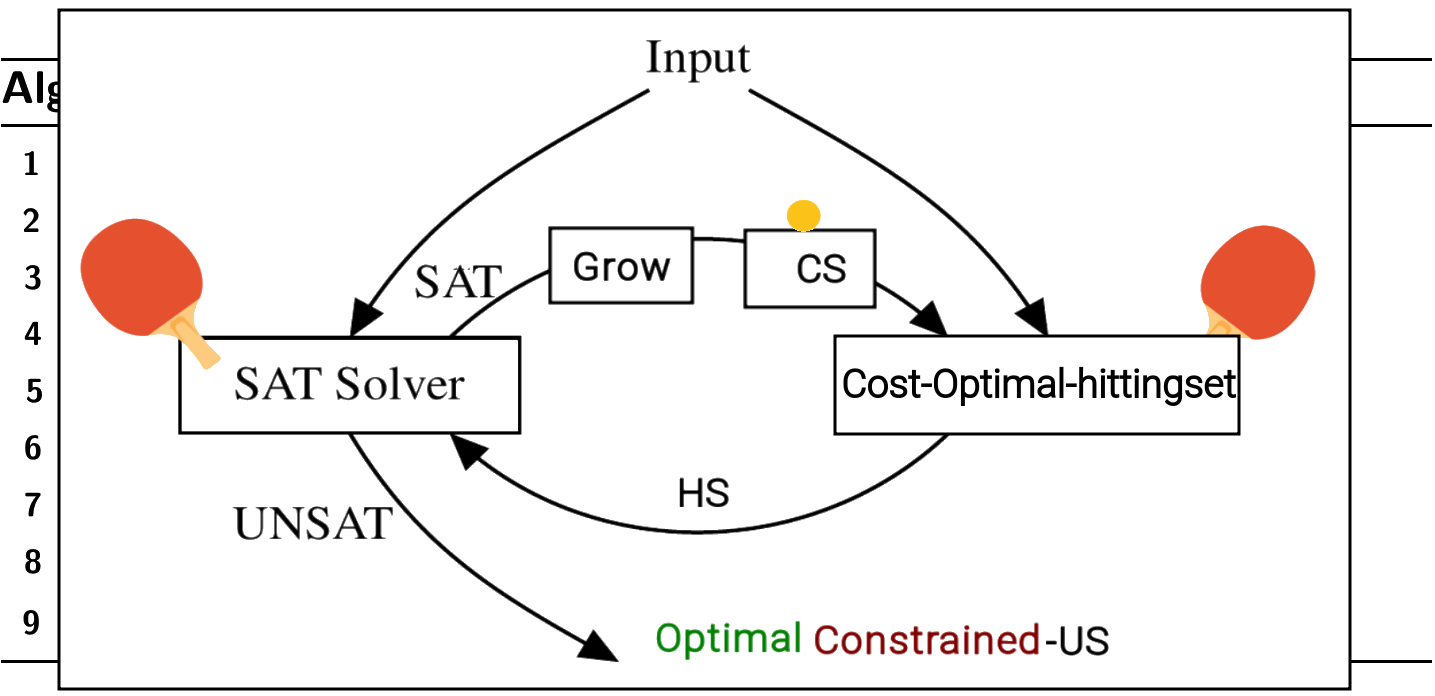
\includegraphics[width=\textwidth]{figures/algo_with_ping_pong2c.png}
	\end{figure}
}
\only<8>{
		\begin{figure}
		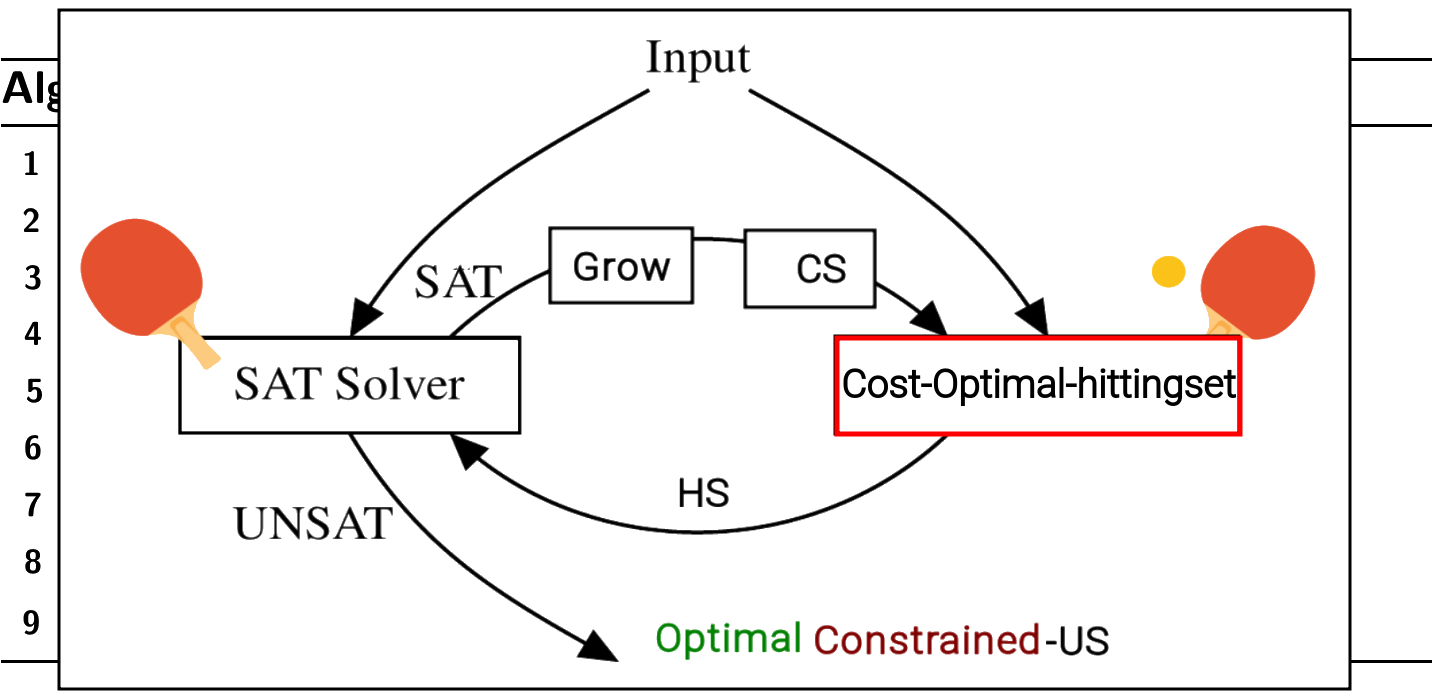
\includegraphics[width=\textwidth]{figures/algo_with_ping_pong.png}
	\end{figure}
}
\only<9>{
		\begin{figure}
		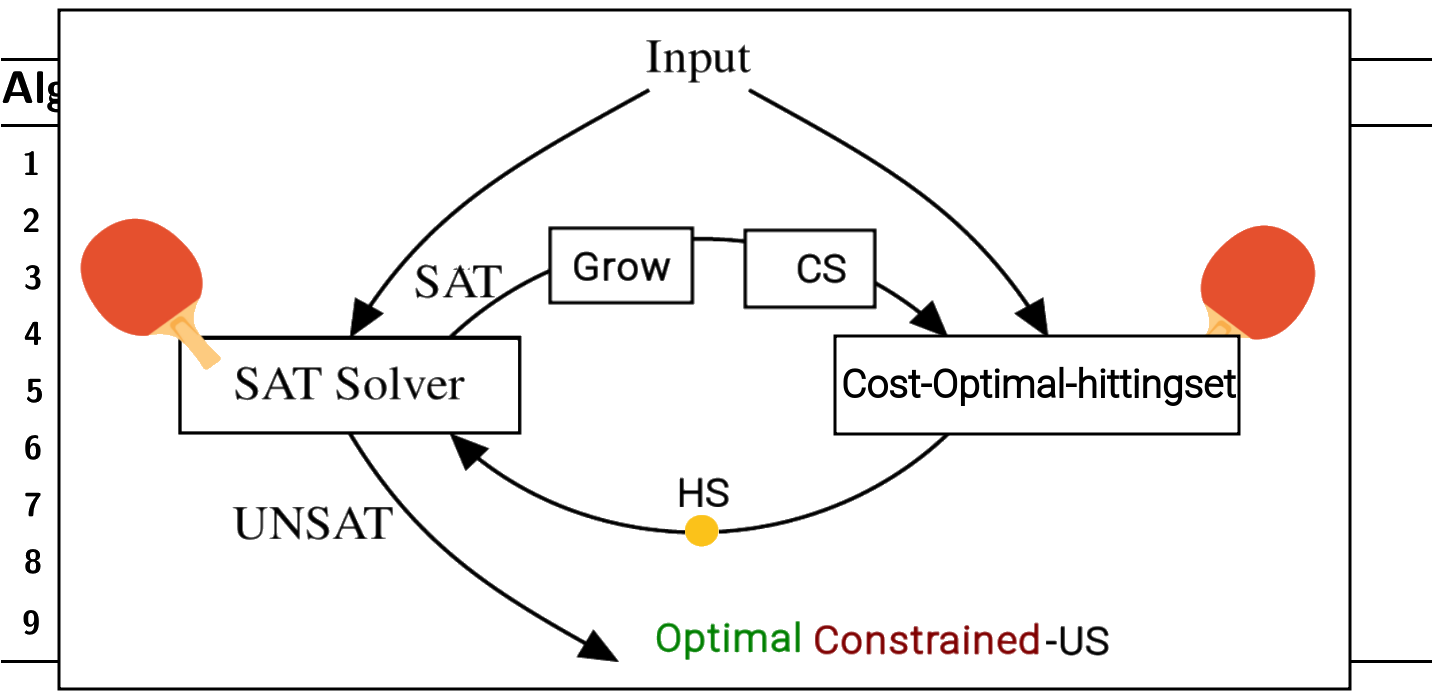
\includegraphics[width=\textwidth]{figures/algo_with_ping_pong1.png}
	\end{figure}
}

\only<10>{
	\begin{figure}
	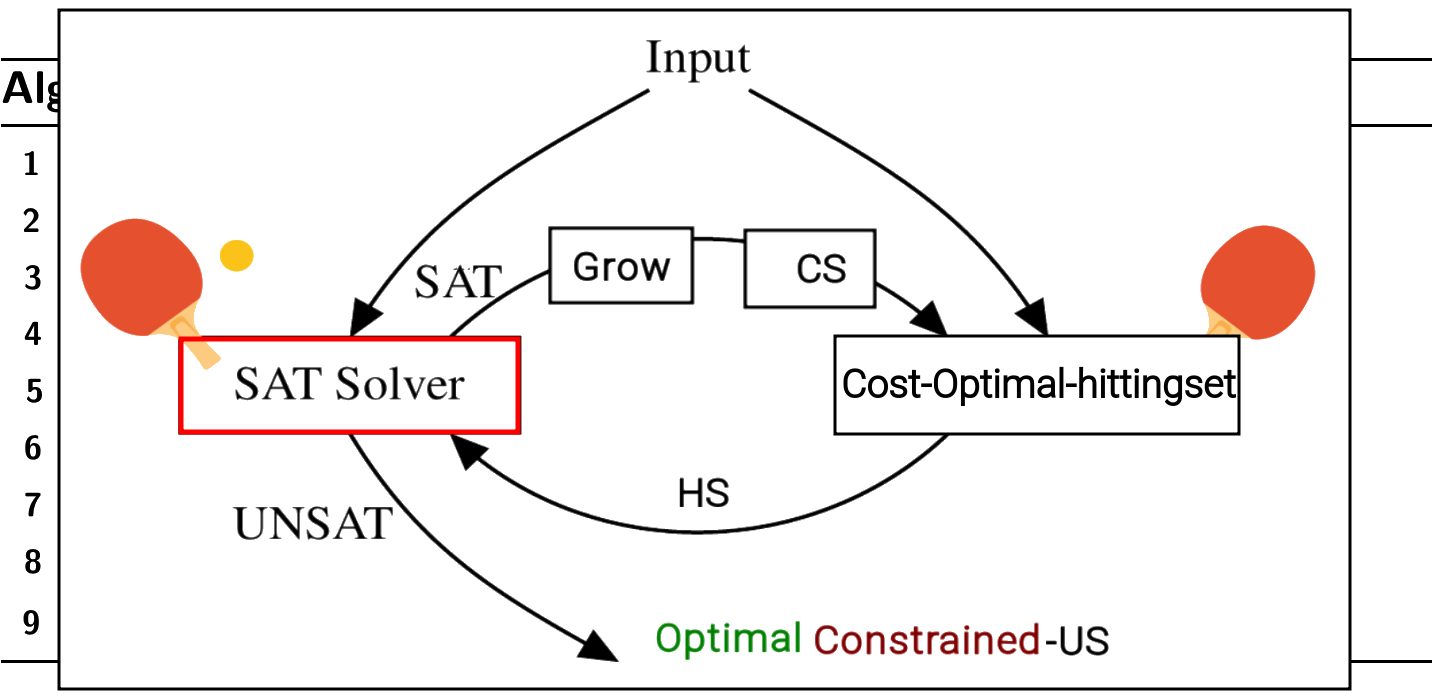
\includegraphics[width=\textwidth]{figures/algo_with_ping_pong2.png}
\end{figure}
}
\only<11>{
	\begin{figure}
	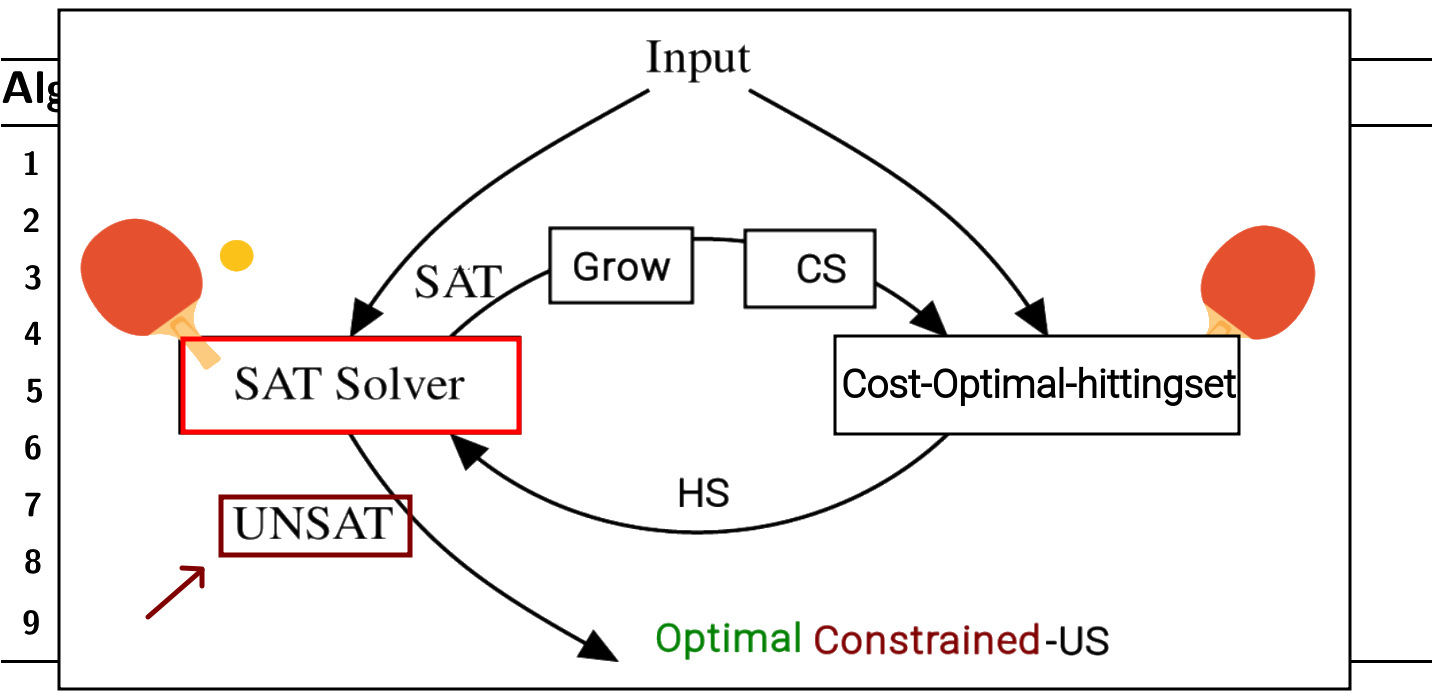
\includegraphics[width=\textwidth]{figures/algo_with_ping_pong2d.png}
\end{figure}
}
\only<12>{
	\begin{figure}
	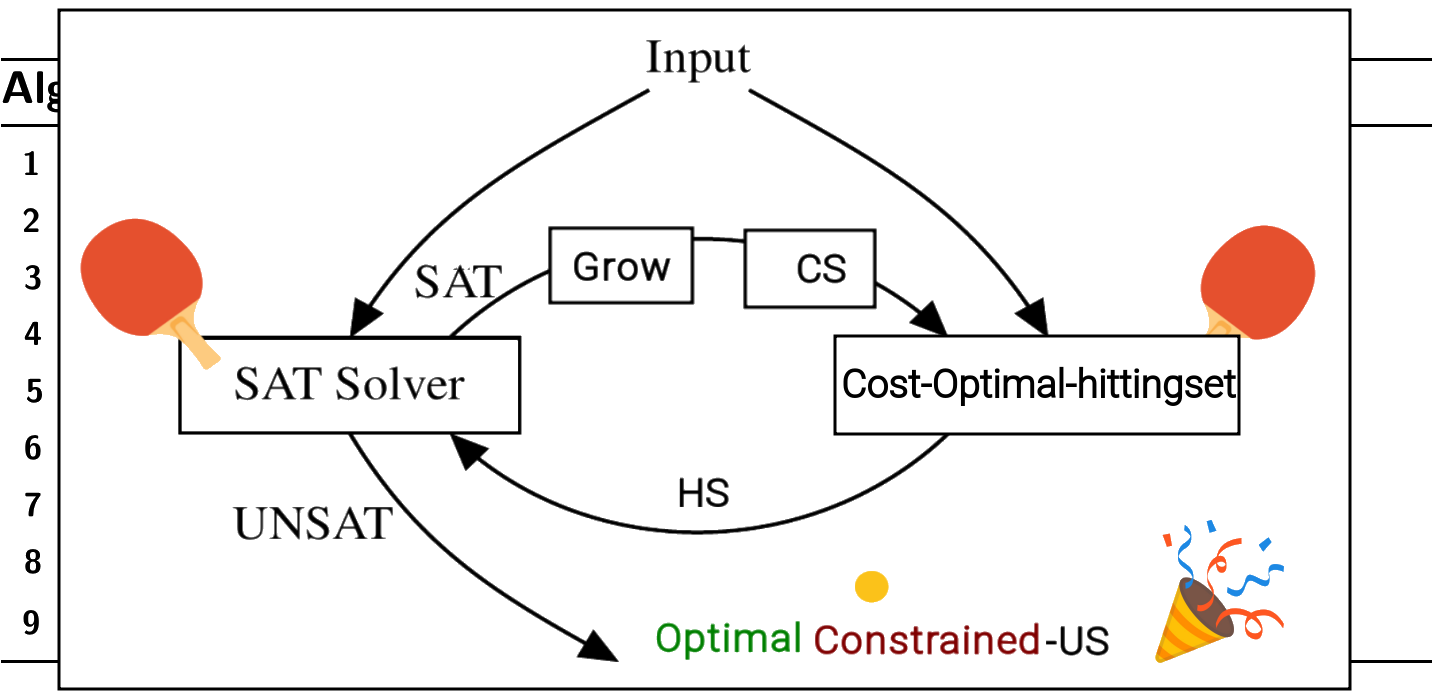
\includegraphics[width=\textwidth]{figures/algo_with_ping_pong3.png}
\end{figure}
}
\newcommand\hitset{\m{\mathcal{H}}}

%\begin{frame}{Correctness}
%	\begin{theorem}\label{thm:soundcomplete}
%		Let $\hitset$ be a set of correction subsets of \formula. 
%		If $\subsetT$ is a hitting set of \hitset that is $f$-optimal among the hitting sets of \hitset satisfying a predicate $p$, and  $\subsetT$ is unsatisfiable, then $\subsetT$ is an OCUS of \formula. 
%		
%		If  $\hitset$ has no hitting sets satisfying $p$, then $\formula$ has no OCUSs.
%	\end{theorem}
\end{frame}


%\subsection{Incrementality}
\subsection{Incrementality}
\begin{frame}{Incrementality}
\framesubtitle{Reusing grown satisfiable subsets}


		$-----(1)------------------(2)------>$\\
		\hspace{1.8cm} $|$ \hspace{6.9cm}$|$
		\[\m{F}_1 := \m{C} \wedge \emph{\m{I}_i} 	\wedge 	\bigvee_{\ell\in \Iend\setminus \emph{\m{I}_i}}\lnot \ell	\hspace{2.8cm}
		 \m{F}_2 :=\m{C} \wedge \emph{\m{I}_{i+1}} \wedge  \bigvee_{\ell\in \Iend\setminus \emph{\m{I}_{i+1}}}\lnot \ell \]

Suppose (1) $\m{F}_1, f_1$ and $ p_1$; and (2) $\m{F}_2, f_2$ and $ p_2$;
\begin{itemize}
	\item Keep track of collection of correction sets $\m{H}$ that need to be hit
	\item Each set H in H is the complement (with respect to the formula at hand) of a satisfiable subset \pause
	\item[$\rightarrow$] Keep track of \emph{set of Satisfiable Subsets \textbf{SSs}} \pause
	\item[$\rightarrow$] Bootstrap $\m{H} \gets \{\m{F}_2 \setminus \m{S} | \m{S}  \in  \mathbf{SSs} \}$ 
\end{itemize}

\end{frame}


\begin{frame}{Incrementality}
	\begin{algorithm}[H]
		\DontPrintSemicolon
		\emph{\bf  $\setstohit  \gets \dots$} \; %\label{omus-line1} 
		\While{\color{black} true}{
			$\subsetT \gets \cohs(\setstohit,f,p) $  \;
			\If{\color{black} $\lnot \sat(\subsetT)$}{
				\Return{\color{black}$\subsetT$} \;
			}
			$\subsetT \gets  \grow(\subsetT,\formula) $ \label{line:grow}\;
			$\setstohit  \gets \setstohit  \cup \{  \formula \setminus \subsetT\}$ \;
		}
		\caption{$\comus(\formula,f,p)$ }
		\label{alg:comus}
	\end{algorithm}
\end{frame}

\subsection{Efficiency}
%\begin{frame}{Optimizations - Improving efficiency}
%	\framesubtitle{Different Grow strategies}
%	\begin{minipage}{.8\textwidth}
%
%	When calling OCUS, the theory consists of 
%	
%	\begin{enumerate}
%		\item The original theory (constraints)\hfill \emph{$\m{C}$}
%		\item The current interpretation\hfill \emph{$\Iend$}
%		\item The negation of literals in $\Iend$  \hfill \emph{$\overline{\Iend}$}
%	\end{enumerate}
%	
%	\begin{itemize}
%		\item What to take into account for \emph{\call{grow}}?
%		\item What about the cost function?
%	\end{itemize}
%	\end{minipage}
%		
%\end{frame}

\begin{frame}{Efficiency}
	\framesubtitle{Explanation specific `Grow'}
	\begin{minipage}{.55\textwidth}
		
		When calling OCUS, the theory consists of 
		
		\begin{enumerate}
			\item[\emph{$\m{C}$}] The original theory (constraints)\hfill 
			\item[\emph{$\Iend$}] The current interpretation\hfill 
			\item[\emph{$\overline{\Iend}$}] The negation of literals in $\Iend$  \hfill 
		\end{enumerate}
		
		\begin{itemize}
			\item What to take into account for \emph{\call{grow}}?
			\item What about the cost function?
		\end{itemize}
	\end{minipage}\hfill
		\begin{minipage}{.4\textwidth}
			{
				\setlength{\algomargin}{0pt}
			\begin{algorithm}[H]
				
				\DontPrintSemicolon
				\bf  $\setstohit  \gets \dots$ \; %\label{omus-line1} 
				\While{\color{black} true}{
					....\;
					$\subsetT \gets COHS(\setstohit,f,p) $  \;
					\If{\color{black} $\lnot \sat(\subsetT)$}{
						\Return{\color{black}$\subsetT$} \;
					}
					$\subsetT \gets  \emph{\grow(\subsetT,\formula)} $ \label{line:grow}\;
					$\setstohit  \gets \setstohit  \cup \{  \formula \setminus \subsetT\}$ \;
				}
				\caption{$\comus(\formula,f,p)$ }
				\label{alg:comus}
			\end{algorithm}
		}
		\end{minipage}
		
	
\end{frame}

\begin{frame}{Bounded OUSs}
	\framesubtitle{Improving efficiency of OUS-based explanations}
	
	\begin{algorithm}[H]
		\caption{$\onestep(\m{C},f,\m{I},\Iend)$}
		\label{alg:oneStep}
		$X_{best} \gets \m{C} \land \m{I} \land \overline{\Iend\setminus \m{I}}$\;
		
		\For{\color{black}$\ell \in \{\Iend \setminus \m{I}\}$}{
			$X \gets \call{OUS}{(\m{C} \land \m{I} \land \neg \ell,f, \emph{f(X_{best})})}$\;
			\If{\color{black}$X \neq null$ and $f(X)<f(X_{best})$}{
				$X_{best} \gets X$\;
			}
		}
		\Return{\color{black}$X_{best}$} 
	\end{algorithm}  \pause
	
	\begin{alertblock}{Bounded OUS computation}
			\small
		In the O(C)US algorithm, if $f(S) > f(X_{best})$, \textbf{STOP}!
		We can't find a better (cheaper) explanation.
	\end{alertblock}
	
\end{frame}


\begin{frame}{Bounded OUSs}
	\framesubtitle{Improving execution time of OUS-based explanations}
	
		\begin{algorithm}[H]
			\caption{$\onestep(\m{C},f,I,\Iend)$}
			\label{alg:oneStep}
			$X_{best} \gets \m{C} \land \m{I} \land \overline{\Iend\setminus \m{I}} $\;
			
			\For{\color{black}$\ell \in \{\Iend \setminus \m{I}\}$}{
				$X \gets \call{OUS}{(\m{C} \land \m{I} \land \neg \ell,f,\emph{ f(X_{best})})}$\;
				\If{\color{black}$X \neq null$ and $f(X)<f(X_{best})$}{
					$X_{best} \gets X$\;
				}
			}
			\Return{\color{black}$X_{best}$} 
		\end{algorithm}
	
	\begin{exampleblock}{}
	\begin{enumerate}	\small
		\item Keep track of the score for all literals not explained yet: serves as an upperbound on explanation cost.\pause
		\item Sort the literals according to their cost.
	\end{enumerate}

	\end{exampleblock}

\end{frame}

\section{Results}
%\begin{frame}{Experiments}
%	\framesubtitle{Research questions}
%  
%	\begin{itemize}	\small
%		\item[Q1] What is the effect of requiring optimality of the generated MUSs on the \textbf{quality} of the generated explanations?
%		\item[Q2] Which \textbf{domain-specific \grow methods} perform best?
%		\item[Q3] What is the effect of the use of \textbf{contrainedness} on the time required to compute an explanation sequence?
%		\item[Q4] Does \textbf{re-use} of computed satisfiable subsets improve efficiency?
%	\end{itemize}
%\end{frame}

\begin{frame}{Results - Explanation quality}
	\centering
	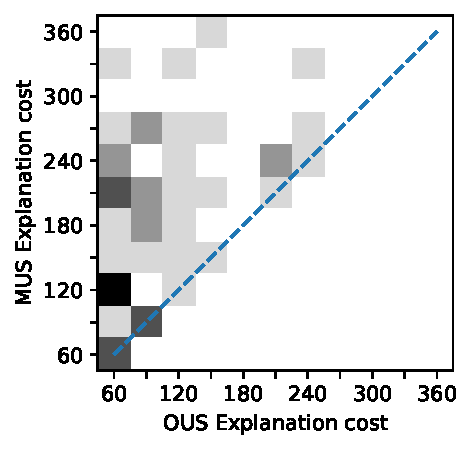
\includegraphics[width=0.6\columnwidth]{figures/rq1_heatmap.pdf}
	
\end{frame}




%	\end{frame}
%
%	\begin{frame}{Incrementality}
%	\framesubtitle{Can we reuse information ?}
%	
%	
%	\end{frame}
%
%	\begin{frame}{Efficiency}
%	
%	
%	\end{frame}


%	\begin{frame}{Motivation}
%		\framesubtitle{Logic Grid Puzzles}
%		\begin{figure}
%			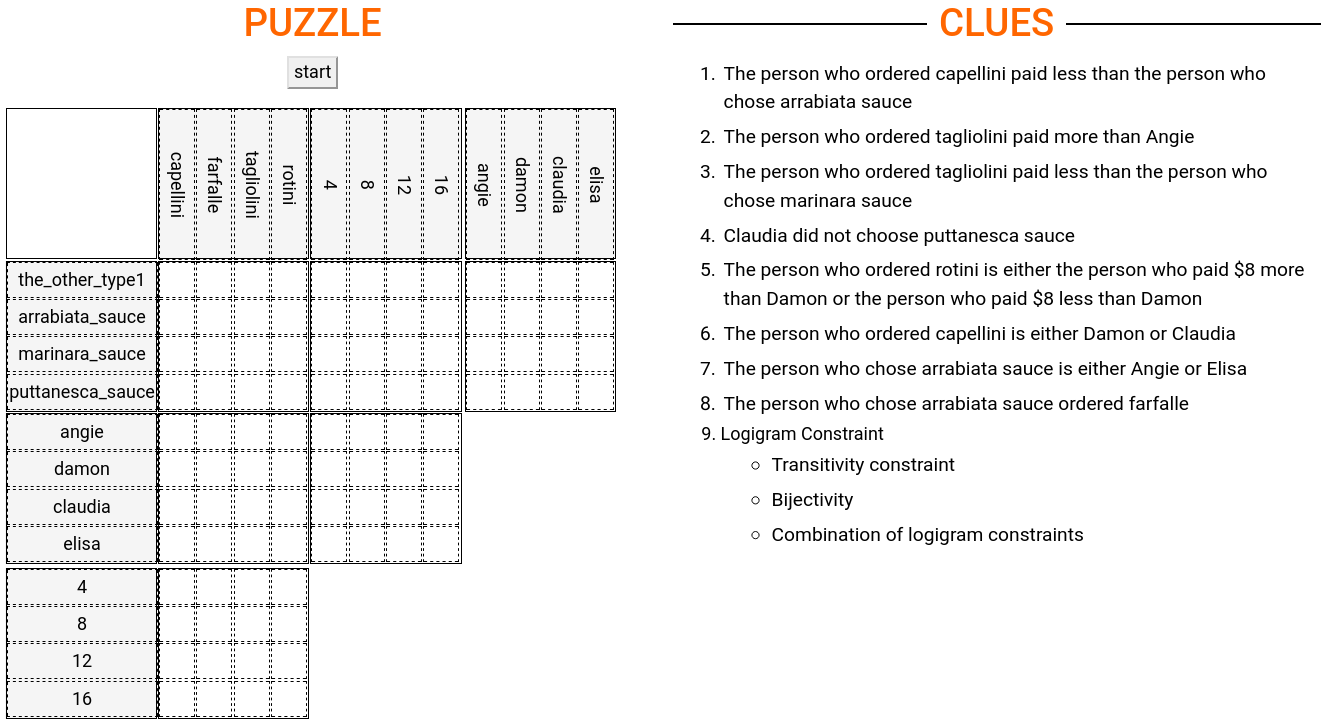
\includegraphics[width=0.9\textwidth]{logicpuzzles.png}
%		\end{figure}
%		\begin{center}
%			\url{https://bartbog.github.io/zebra/pasta/}
%		\end{center}
%	\end{frame}
%	
%	\begin{frame}{Motivation}
%		\framesubtitle{CSPs: a little formal Background}
%		
%		\begin{itemize}
%			%               \setlength{\leftmargin}{0pt}
%			\item[$\m{C}$] \emph{constraints} we can use to reason (alldifferent, George did not take pasta, …)
%			\item[$\mathcal{I}_0$] an \emph{Initial Interpretation}
%			\item[$\mathcal{I}_{end}$] Everything we can derive from $ \m{C} \wedge \mathcal{I}_0$
%		\end{itemize}
%		\begin{figure}
%			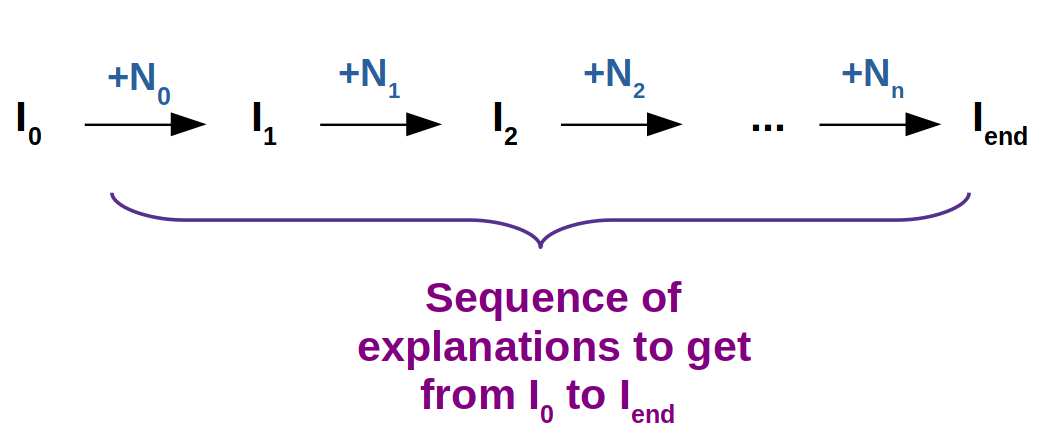
\includegraphics[width=0.7\textwidth]{sequence_explanation.png}
%		\end{figure}
%	\end{frame}
%	
%	
%	\begin{frame}{Motivation}
%		\framesubtitle{Gentle reminder: Explanations for CSPs}
%		\begin{definition}
%			Given one or a subset of the constraints ( $S_i \subseteq T_P$  ) and facts we know ($E_i\subseteq \mathcal{I}_i$), an \textbf{explanation} is an implication of the form $E_i \wedge S_i  \implies N_i $, where $N_i$ is the new information from $S_i \cup E_i \models N_i$. \cite{bogaerts2020step}
%		\end{definition}
%		
%	\end{frame}
%	
%	\begin{frame}{Motivation}
%		\begin{figure}
%			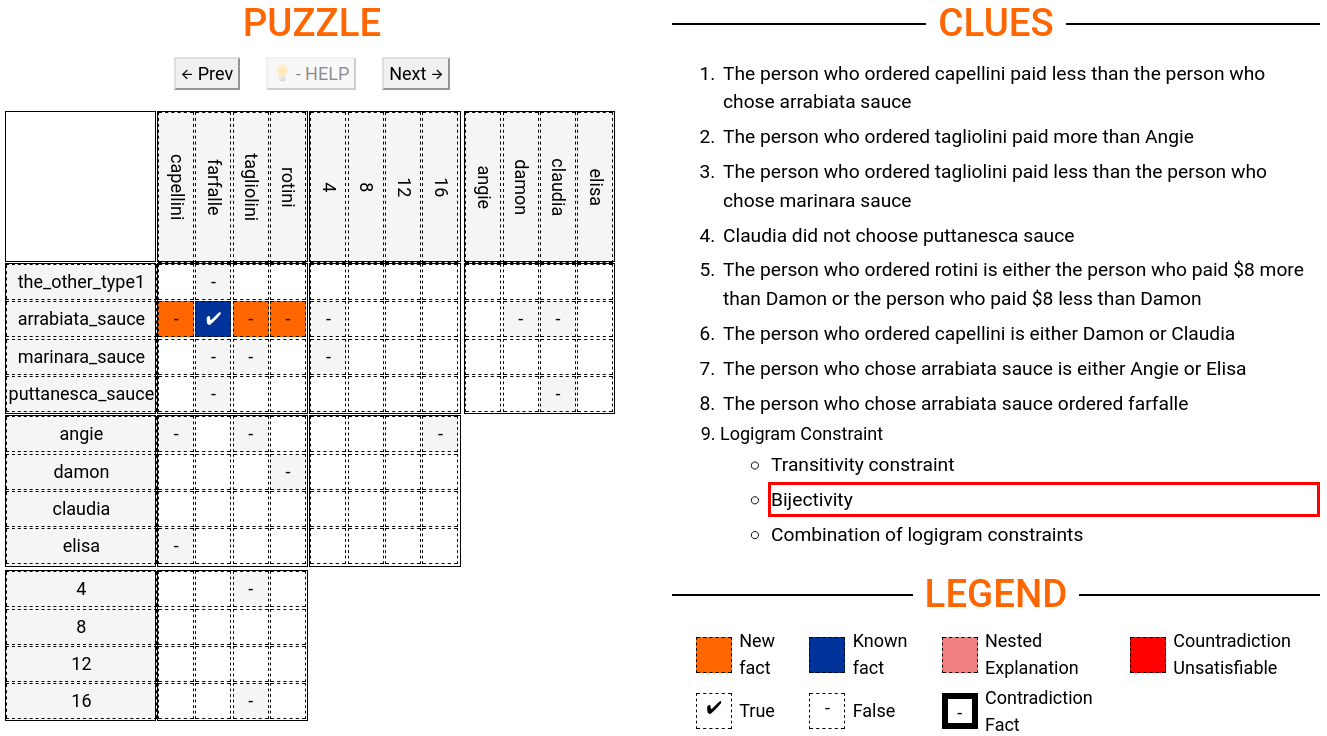
\includegraphics[width=0.8\textwidth]{logic_puzzles_bij.png}
%		\end{figure}\pause
%		\begin{itemize}
%			\item[$E_i$] farfalle goes with arrabiata sauce \pause
%			\item[$S_i$] an entity of type pasta can only be linked to one entity of type sauce\pause
%			\item[$N_i$] taglioni, rotini and capellini cannot be linked to arriabiata
%		\end{itemize}
%		
%	\end{frame}
%	
%	\newcommand\onestep{\ensuremath{\call{explain-One-Step}}\xspace}
%	
%		\begin{frame}{Motivation}
%		\framesubtitle{Gentle reminder: Explanations for CSPs}
%		\begin{definition}
%			Given one or a subset of the constraints ( $S_i \subseteq T_P$  ) and facts we know ($E_i\subseteq \mathcal{I}_i$), an \textbf{explanation} is an implication of the form $E_i \wedge S_i  \implies N_i $, where $N_i$ is the new information from $S_i \cup E_i \models N_i$. \cite{bogaerts2020step}
%		\end{definition} 
%		
%		An \textbf{explanation sequence} is of the form $$<(\mathcal{I}_0,(\emptyset,\emptyset,\emptyset)),\text{\hspace{3pt}}(\mathcal{I}_1,(E_1, S_1, N_1)),\text{\hspace{3pt}}...,\text{\hspace{3pt}}(\mathcal{I}_{end},(E_{n}, S_n, N_n ))>$$
%		
%		\begin{figure}
%			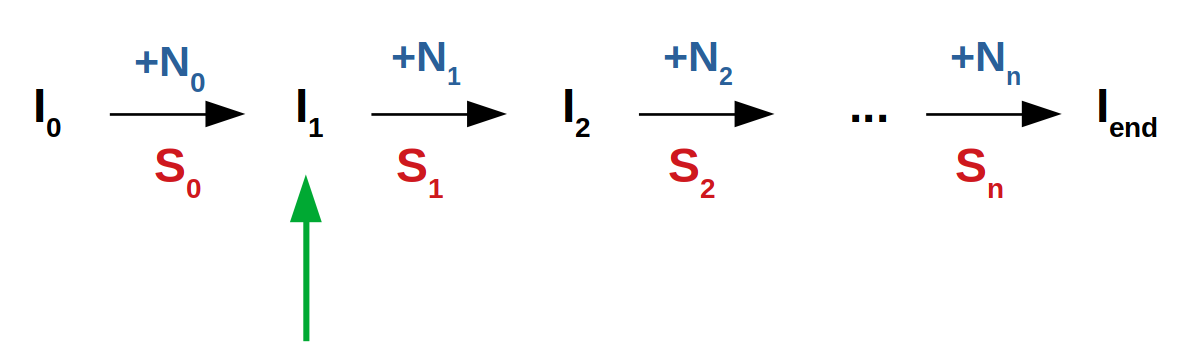
\includegraphics[width=0.7\textwidth]{sequence_explanation2.png}
%		\end{figure}
%		
%	\end{frame}
%	
%	\begin{frame}{Motivation}
%		\framesubtitle{Generating an explanation sequence for CSPs}
%\cite{bogaerts2020step}: At every step in the explanation sequence:
%		\begin{figure}
%			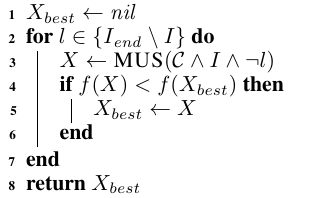
\includegraphics[width=0.45\textwidth]{algo_mus2.png}
%		\end{figure}
%		\begin{itemize}
%			\item Finding non-redundant explanations: MUS($\formulac \land \mathcal{I} \land \neg l$) extraction (IDP system)
%			
%		\end{itemize}
%	\end{frame}
%
%	\begin{frame}{Motivation}
%	\framesubtitle{Generating an explanation sequence for CSPs}
%\cite{bogaerts2020step}: At every step in the explanation sequence:
%	\begin{figure}
%		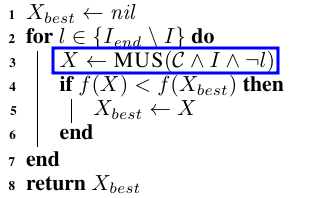
\includegraphics[width=0.45\textwidth]{algo_mus2_b.png}
%	\end{figure}
%	\begin{itemize}
%		\item Finding non-redundant explanations: MUS($\formulac \land \mathcal{I} \land \neg l $) extraction (IDP system)
%		
%		\begin{itemize}
%			\item In practice, not all constraints at once!
%			\item Consider power sets of constraints sorted by increasing cost
%		\end{itemize}
%	\end{itemize}
%\end{frame}
%
%	
%	\begin{frame}{Motivation}
%		\framesubtitle{Open Questions}
%		
%		\begin{description}[font=\color{vuborange}\itshape]
%			\item[\hspace{0.9cm}Optimality] Explanations not optimal, heuristically found \pause
%			\item[\hspace{1.05cm}Efficiency] Explanation generation takes a lot of time \pause
%			\item[\hspace{0.3cm}Incrementality] Can we reuse information from an explanation call to another? \pause
%			\item[Constrainedness] Can we avoid looping over the literals when searching for the next best explanation ?
%		\end{description}
%	\end{frame}
%	
%	\begin{frame}{Optimality}
%		\pause
%		\begin{minipage}{0.49\textwidth}
%						\begin{figure}
%				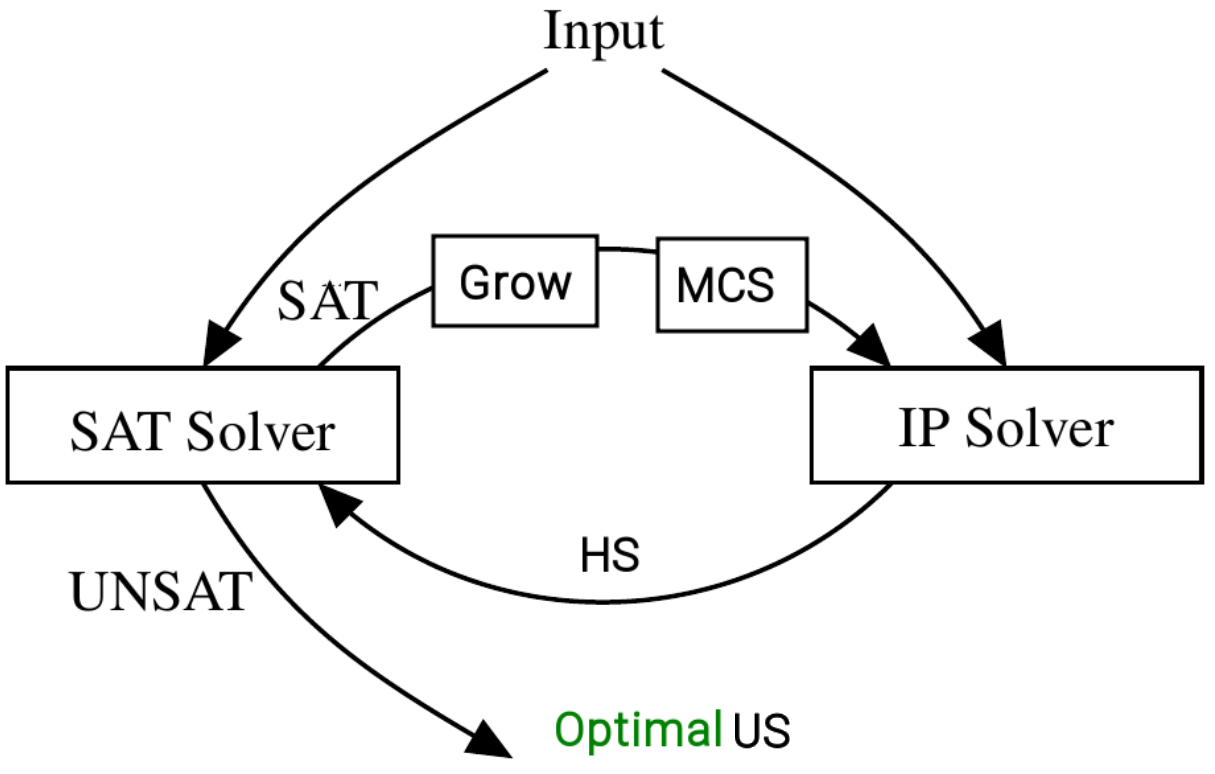
\includegraphics[width=\textwidth]{ihs.png}
%			\end{figure}
%			\pause
%		\end{minipage}
%		\begin{minipage}{0.5\textwidth}
%		\begin{itemize}
%			\item Inspired by \cite{ignatiev2015smallest}
%			\item MIP solver instead of SAT-based
%			\item[+] Optimal Hitting set (\emph{\textbf{Optimality}})
%		\end{itemize}
%		\end{minipage}
%		\vfill
%		\begin{figure}
%			
\includegraphics[width=\textwidth]{mus_to_ous.png}
%		\end{figure}
%		
%	\end{frame}
%
%\begin{frame}{Optimality}
%	\framesubtitle{Verifying explanation quality}
%	\pause
%			\begin{figure}
%		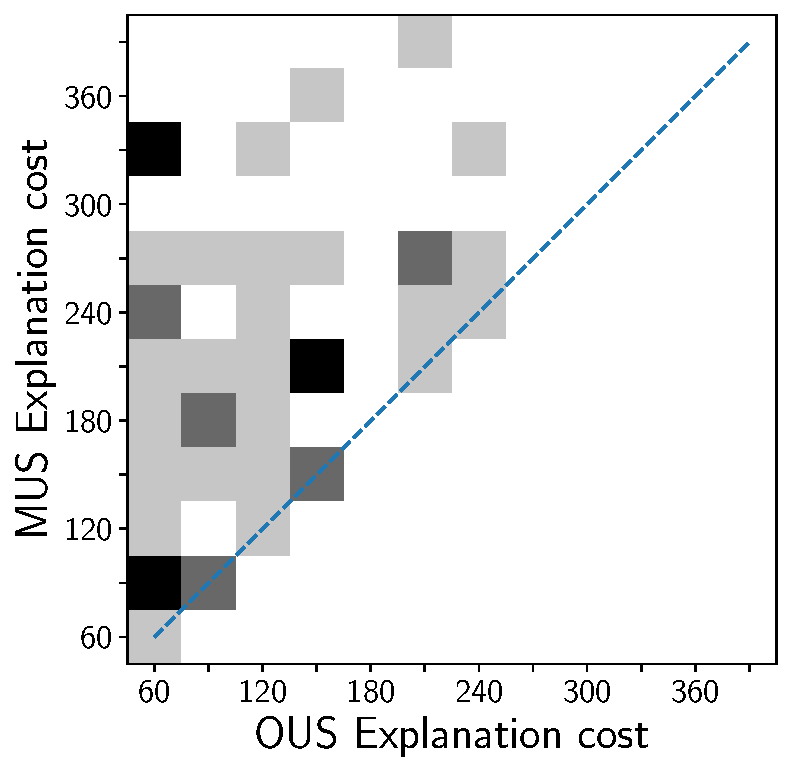
\includegraphics[width=0.6\textwidth]{heatmap_costs_mus_cous.pdf}
%	\end{figure}
%\end{frame}
%	
%	
%	
%	
%		\begin{frame}{Incrementality}
%			\framesubtitle{Improving efficiency of OUS}
%		
%		\begin{minipage}{0.59\textwidth}
%			\begin{enumerate}
%				\item {\color{vuborange} Incremental \emph{OUSs} }
%				\begin{itemize}
%					\item Keep Satisfiable Subsets between OUS-calls
%				\end{itemize}	
%			\end{enumerate}
%		\end{minipage}
%		\begin{minipage}{0.4\textwidth}
%			\begin{figure}
%				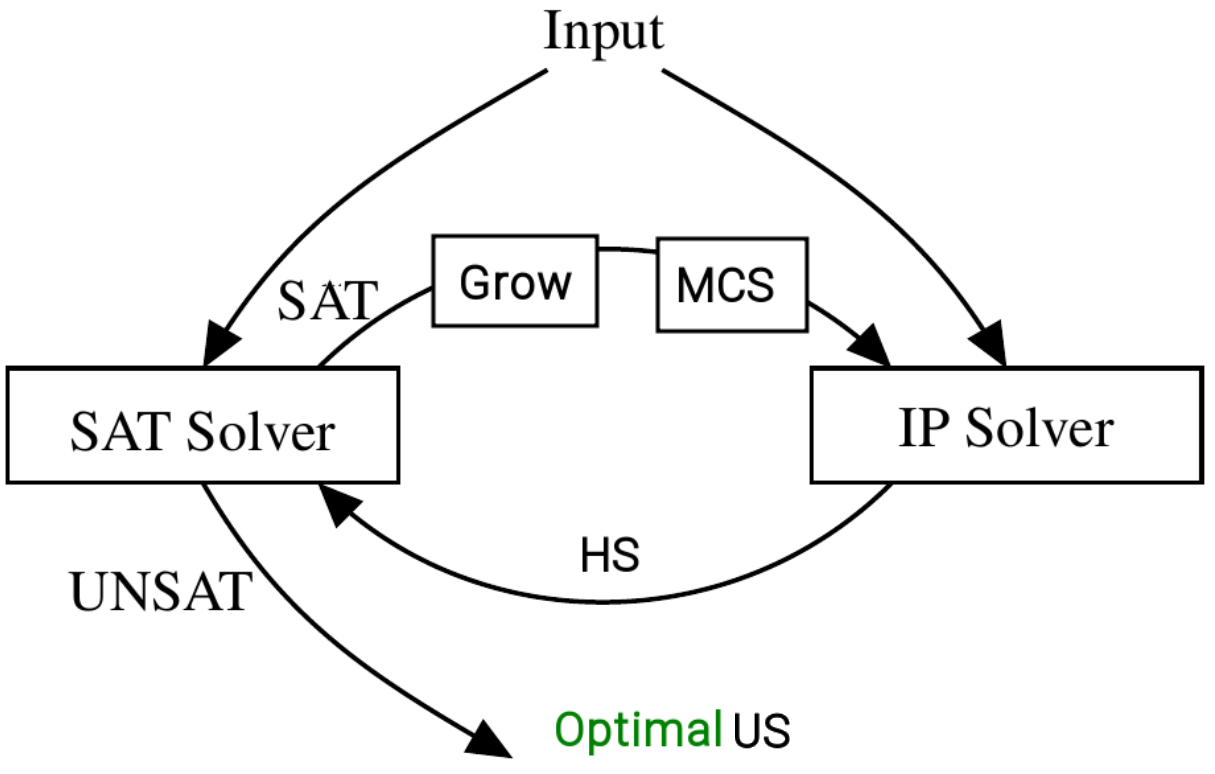
\includegraphics[width=\textwidth]{ihs.png}
%			\end{figure}
%		\end{minipage}
%		\vfill
%		\begin{figure}
%			
\includegraphics[width=\textwidth]{mus_to_ous_i.png}
%		\end{figure}
%	\end{frame}
%	
%	
%	
%	\begin{frame}{Incrementality}
%		
%		\begin{minipage}{0.59\textwidth}
%			\begin{enumerate}
%				\item {\color{vuborange} Incremental \emph{OUSs} }
%				\begin{itemize}
%					\item Keep Satisfiable Subsets between OUS-calls
%					\item Naïve OUS-restart $\rightarrow$ Keep 1 MIP solver warm per literal
%					\begin{itemize}
%						\item[$\implies$] No need to keep track of Satisfiable Subsets
%					\end{itemize}
%				\end{itemize}	
%			\end{enumerate}
%		\end{minipage}
%		\begin{minipage}{0.4\textwidth}
%			\begin{figure}
%				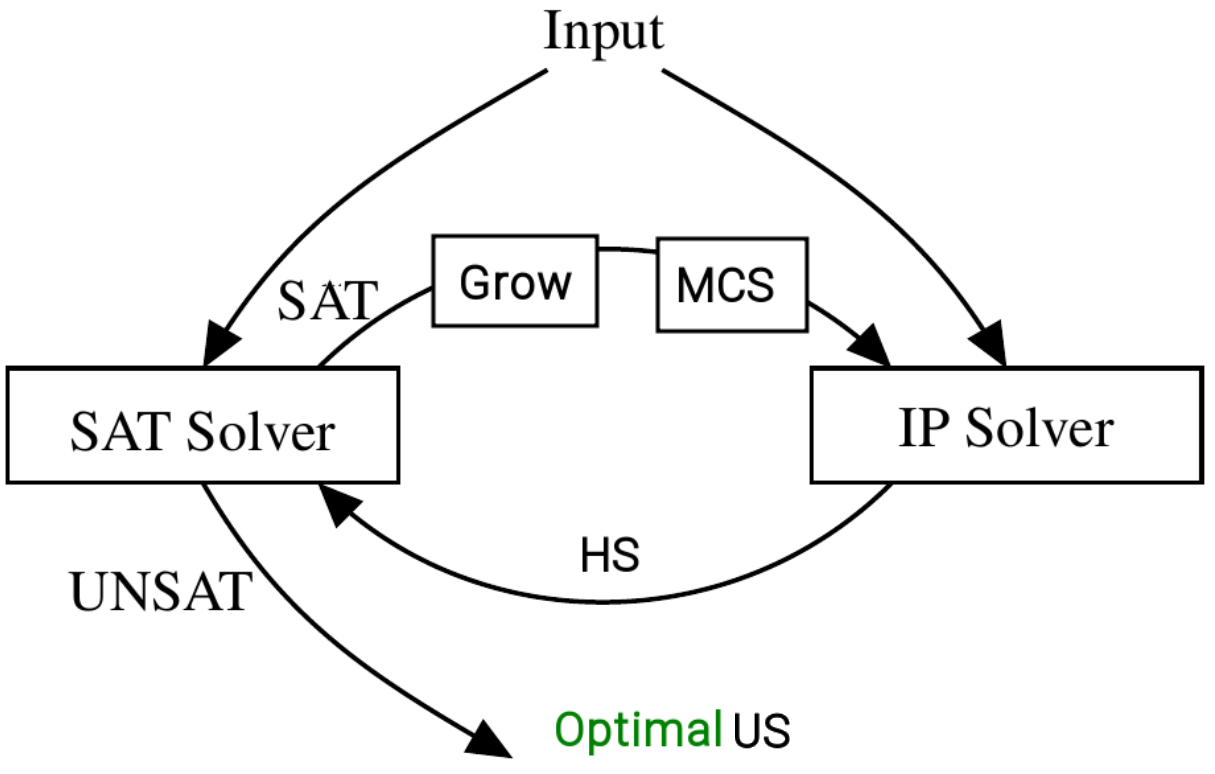
\includegraphics[width=\textwidth]{ihs.png}
%			\end{figure}
%		\end{minipage}
%	\vfill
%		\begin{figure}
%		
\includegraphics[width=\textwidth]{mus_to_ous_i_litincr.png}
%	\end{figure}
%	\end{frame}
%
%	\begin{frame}{Incrementality}
%	
%	\begin{minipage}{0.59\textwidth}
%		\begin{enumerate}
%			\item {\color{vuborange} Incremental \emph{OUSs}}
%			\begin{itemize}
%				\item Keep Satisfiable Subsets between OUS-calls
%				\item Naïve OUS-restart $\rightarrow$ Keep 1 MIP solver warm per literal
%				\begin{itemize}
%					\item[$\implies$] No need to keep track of Satisfiable Subsets
%				\end{itemize}
%			\end{itemize}	
%		\end{enumerate}
%	\end{minipage}
%	\begin{minipage}{0.39\textwidth}
%		\begin{figure}
%			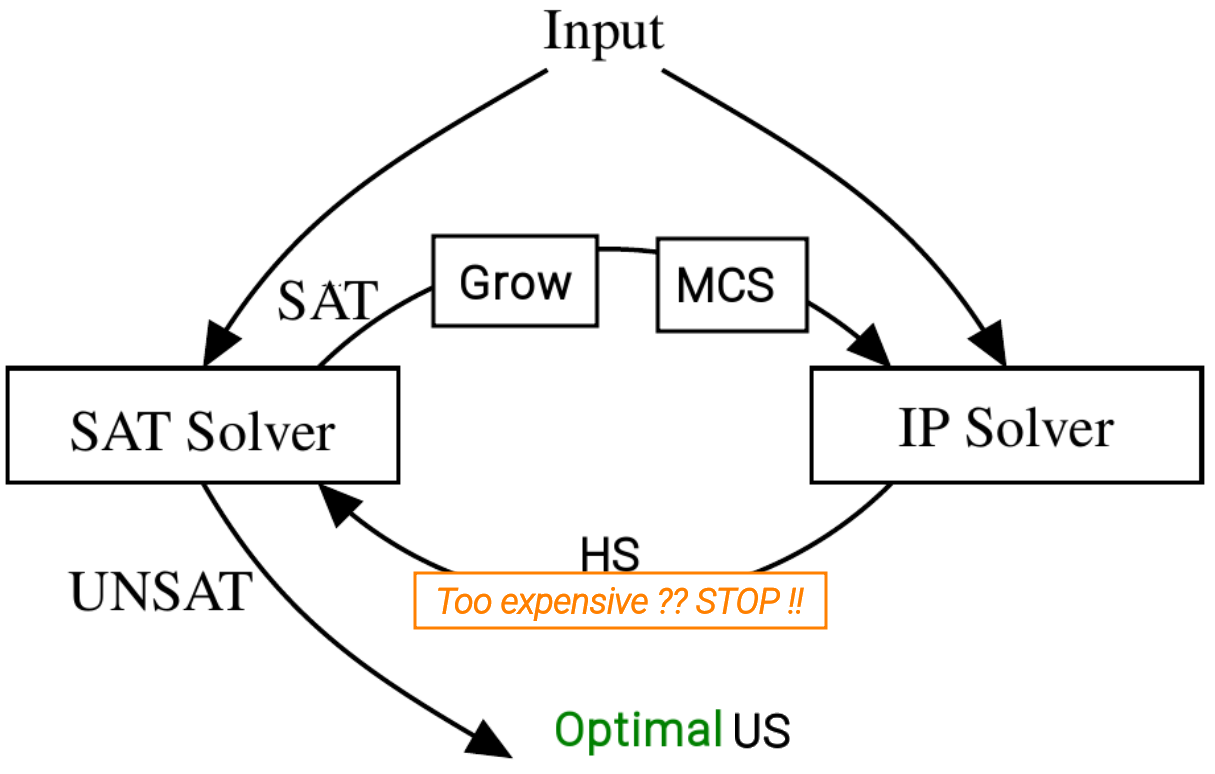
\includegraphics[width=\textwidth]{ihs_cost.png}
%		\end{figure}
%	\end{minipage}
%	\begin{enumerate}
%		\item {\color{vuborange} + Optimizations {\color{blue} (Bounded)}}
%		\begin{itemize}
%			\item Keep track of cost for computed OUSs 
%			\begin{itemize}
%				\item[$\implies$] Use previously found bound on OUS to interrupt if cost(HS) too high 
%			\end{itemize}
%			\item Sort the literals based on cost
%		\end{itemize}
%	\end{enumerate}
%	
%	\begin{figure}
%		
\includegraphics[width=\textwidth]{mus_to_ous_i_bounded.png}
%	\end{figure}
%\end{frame}
%
%\begin{frame}{Optimality \& Constrainedness}
%	\begin{figure}
%		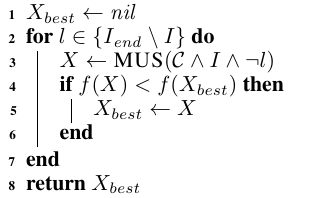
\includegraphics[width=0.45\textwidth]{algo_mus2.png}
%	\end{figure}\pause
%	{\Huge$$\downarrow$$}
%	\begin{figure}
%		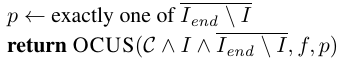
\includegraphics[width=0.5\textwidth]{exactly_one.png}
%	\end{figure}
%\end{frame}
%
%\begin{frame}{Optimality \& Constrainedness}
%	\begin{minipage}{0.49\textwidth}
%		\begin{figure}
%			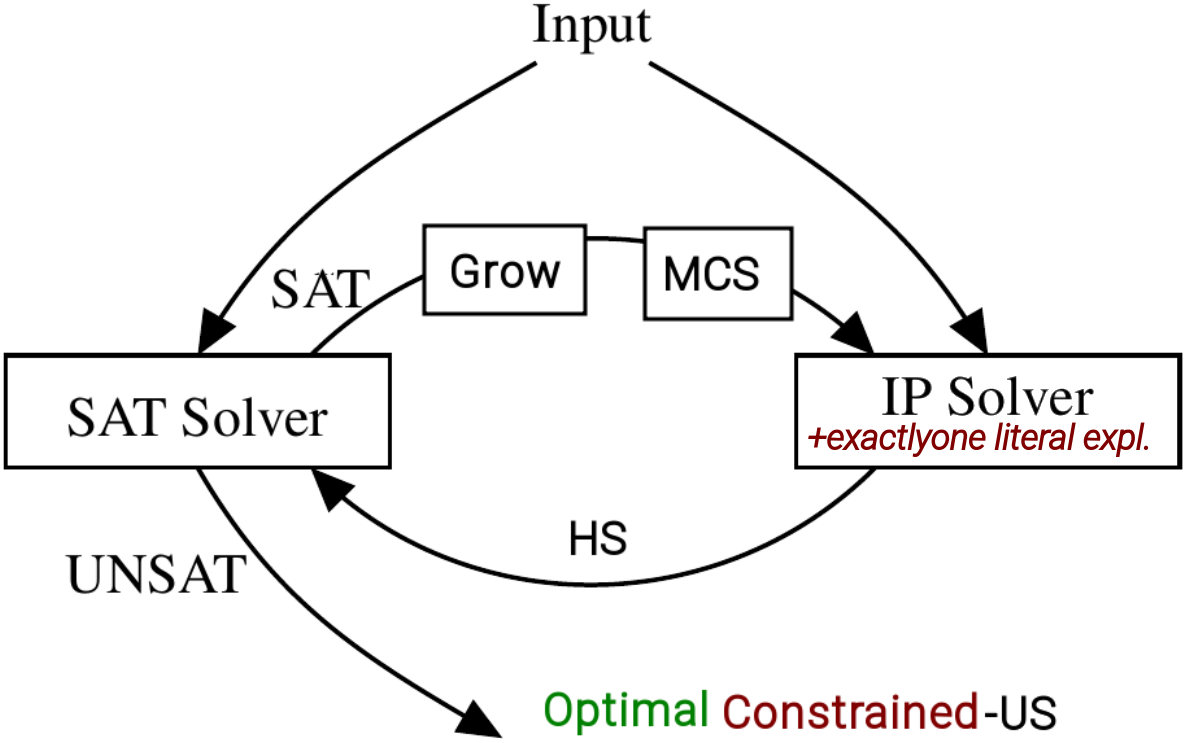
\includegraphics[width=\textwidth]{ihs_constrained.png}
%		\end{figure}
%	\end{minipage}
%	\begin{minipage}{0.5\textwidth}
%		% TODO: ADD algorithm  one step !
%		\begin{itemize}
%			\item Inspired by \cite{ignatiev2015smallest}
%			\item MIP solver instead of SAT-based
%			\item[+] Optimal Hitting set (\emph{\textbf{Optimality}})
%			\item[+] {\color{red} 1 literal explained (\emph{\textbf{Constrained}})}
%		\end{itemize}
%	\end{minipage}
%	\vfill
%	\begin{figure}[h]
%		
\includegraphics[width=\textwidth]{mus_to_ocus.png}
%	\end{figure}
%	
%\end{frame}
%
%\begin{frame}{Optimality \& Constrainedness + Incrementality}
%		\begin{enumerate}
%			\item \color{vuborange} Incremental \emph{OUSs} + optimizations {\color{blue} (Bounded)}\pause
%			\item {\color{vuborange} Incremental \emph{OCUS}}
%			\begin{itemize}
%				\item Naïve OCUS-restart $\rightarrow$ Keep only 1 MIP solver warm
%			\end{itemize}
%		\end{enumerate}
%		\begin{figure}
%			
\includegraphics[width=\textwidth]{mus_to_ocus_i.png}
%		\end{figure}
%	\end{frame}

%\section{Experiment}
\begin{frame}{Results - Constrainedness and Incrementality}
%	\framesubtitle{Explanation configurations compared}
	\begin{figure}
		\includegraphics[width=0.9\textwidth]{figures/cumul_incr_avg_time_lits_derived_new_annotated.pdf}
	\end{figure}
\end{frame}

\begin{frame}{Results - Explanation specific grow}
	%	\framesubtitle{Explanation configurations compared}
	\begin{figure}
		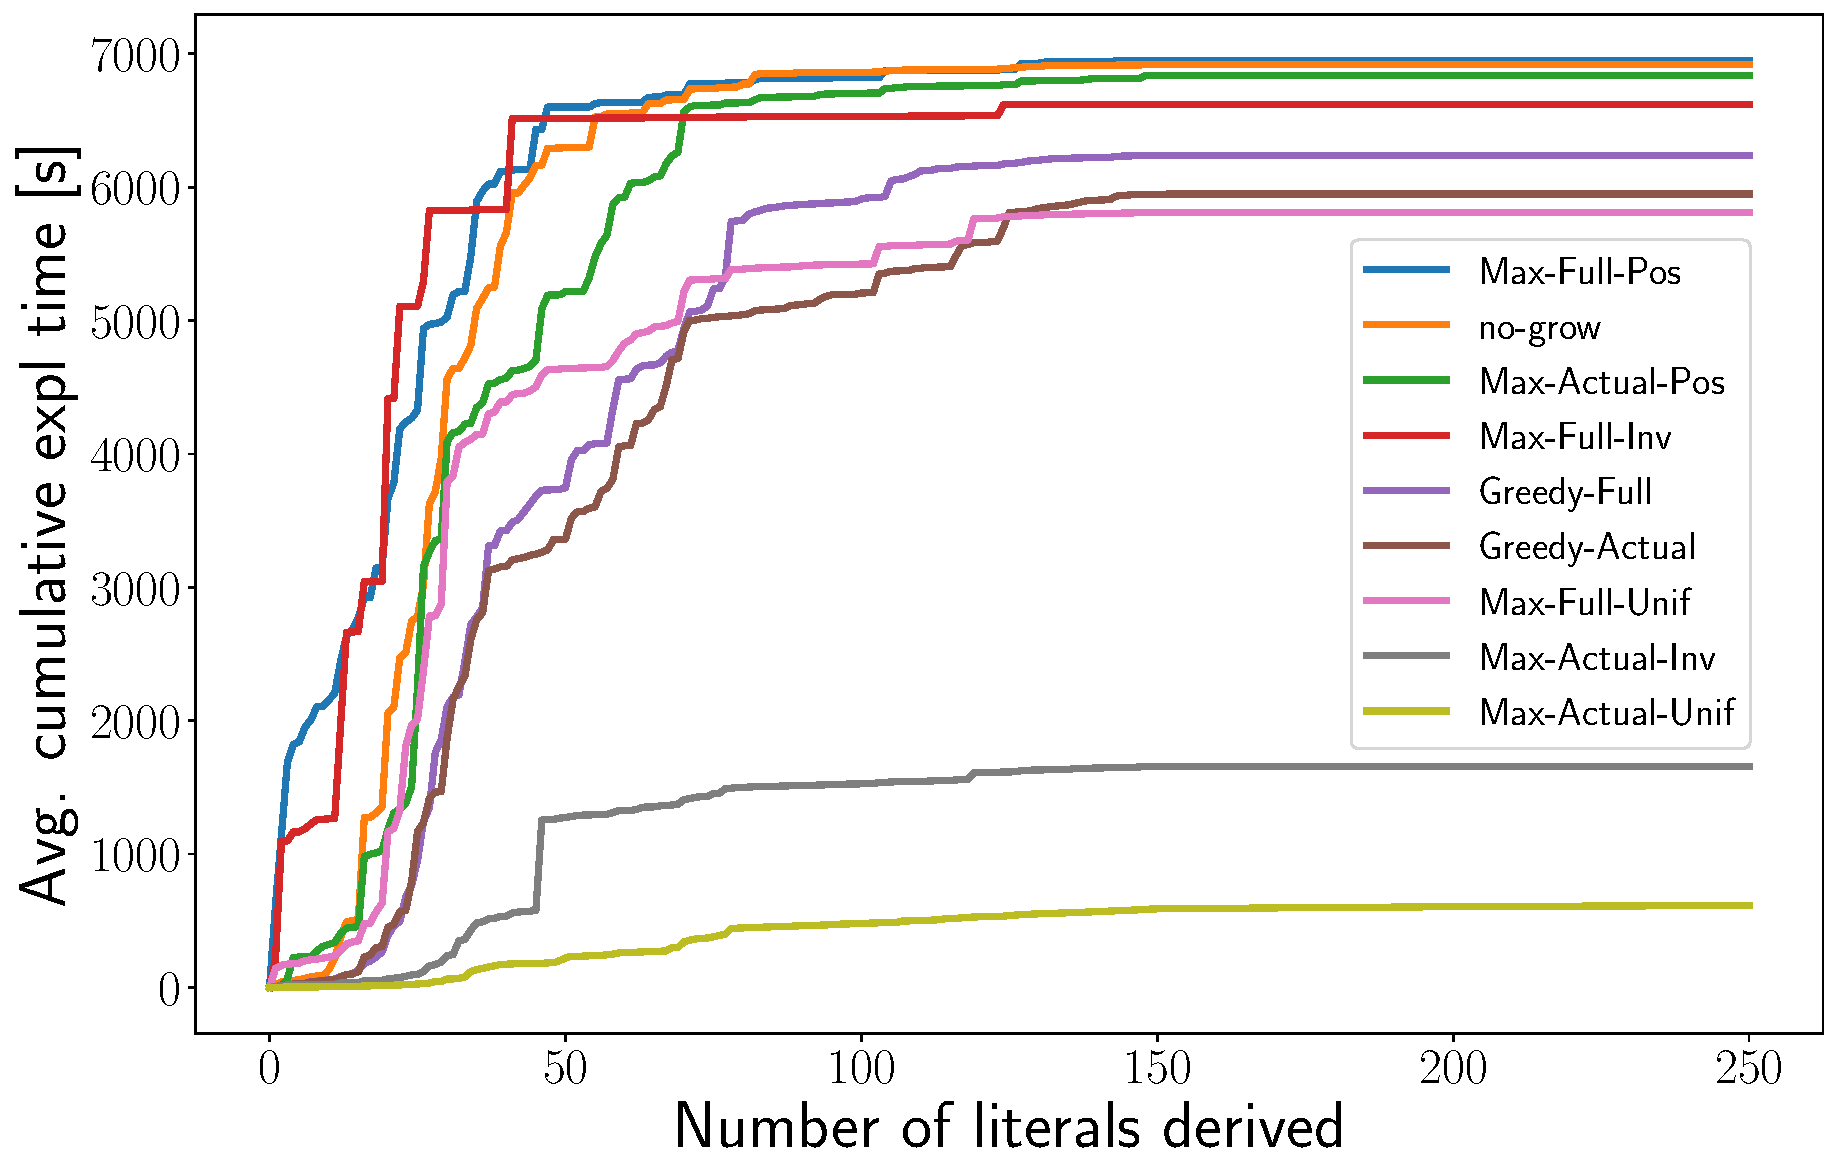
\includegraphics[width=0.9\textwidth]{figures/new_cumul_grow_avg_time_lits_derived_new.pdf}
	\end{figure}
\end{frame}

\section{Conclusion, Use Cases and Future work}
\begin{frame}{Conclusion}
	In this paper, we introduce (cost-)\textbf{\underline{O}ptimal} \underline{U}nsatisfiable \underline{S}ubsets (OUS) using the \emph{implicit hitting set duality}.
	\begin{description}
		\item[Optimality] Cost-function quantifies explanation difficulty. \pause
		\item[Constrainedness] Analyze structural constraints on the form of the explanations.\pause
		\item[Incrementality] Reuse-information between successive explanation calls.\pause
		\item[Efficiency] 
		\begin{enumerate}
			\item Explanation-specific grow;
			\item Bound and sort OUS calls
		\end{enumerate}
		
%		(1)  (2)  to improve time to find the next best explanation.\pause
	\end{description}
%	\vfill
\end{frame}
	\begin{frame}{Use Cases}
%	\framesubtitle{}
	\begin{minipage}{0.6\textwidth}
		 \begin{itemize}
			\item Teach humans how to solve a certain problem
			\item Quantify problem difficulty
			\item ``Help'' button
			\item Interactive configuration/planning/scheduling
		\end{itemize}
		
	\end{minipage}
	\begin{minipage}{0.39\textwidth}
		\begin{figure}
			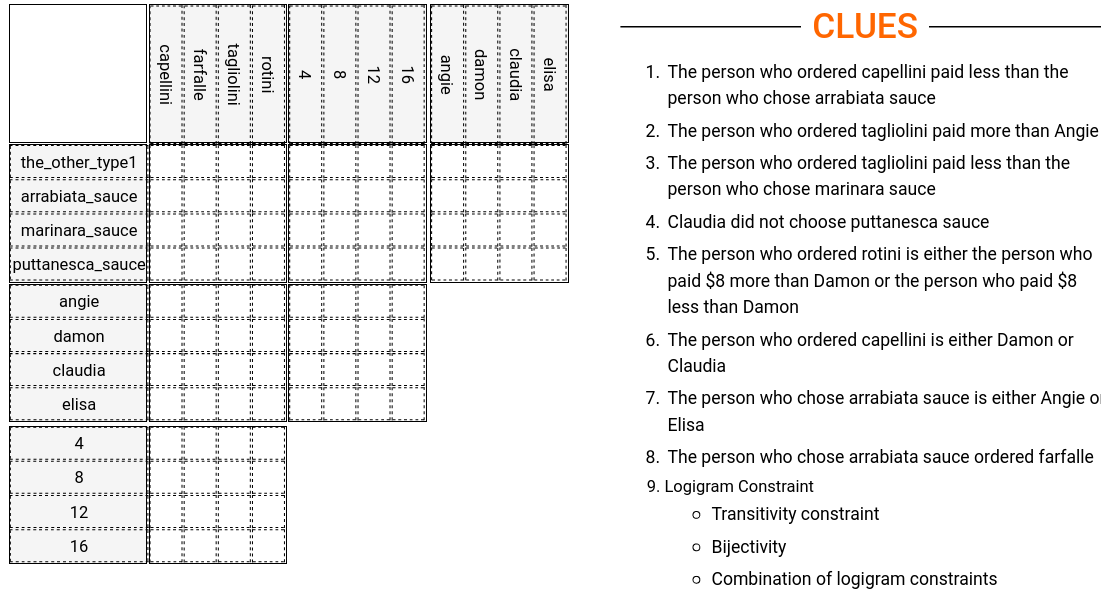
\includegraphics[width=\textwidth]{figures/logic_puzzle.png}
		\end{figure}
	\end{minipage}

	
	
\end{frame}

	\begin{frame}{Future work}

\begin{itemize}
	%  \item Unsat-core optimization
	\item Learning the optimization function (from humans)
	%  \item Nested explanation sequences
	\item Explaining optimization (different types of ``why'' queries); close relation to Explainable AI Planning \cite{fox2017explainable}
	\item Scaling up (approximate algorithms; decomposition of explanation search)
	\item Incremental algorithms over different ``why'' queries
	% \item 
\end{itemize}	
	
	
\end{frame}


	\begin{frame}
		\begin{center}
			{\huge Questions?}
		\end{center}
%		\begin{itemize}
%			\item \href{mailto:emilio.gamba@vub.be}{\underline{emilio.gamba@vub.be}}
%%			\item \href{https://arxiv.org/abs/2105.11763}{\emph{Link to paper}}
%%			\item \href{}{\emph{2 minute talk recording}}
%%			\item \href{}{\emph{15 minute talk recording}}
%		\end{itemize}

		
		
	\end{frame}

	
	\begin{frame}[allowframebreaks]
		\frametitle{References}
		\bibliographystyle{named}
		\bibliography{refs}
	\end{frame}
	

	
\end{document}